\documentclass{sig-alternate-10pt}

\usepackage[breaklinks=true,colorlinks=true,plainpages=false,citecolor=blue,urlcolor=blue,linkcolor=magenta,filecolor=blue]{hyperref}
\usepackage{url}        % Not compatible with hyperref?
\usepackage{float}
\usepackage{graphicx}
\usepackage{amsmath}
\usepackage{color}
\usepackage{times}
\usepackage[sort]{natbib}
\usepackage{enumitem}
%\usepackage{subfigure}
\usepackage{verbatim}
\usepackage{xspace}
\usepackage{xfrac}
\usepackage{algorithmic} % must come after hyperref
\usepackage{algorithm}
%ejr ac/dc 
\usepackage{marvosym}
\let\marvosymLightning\Lightning

\usepackage{lastpage}

\usepackage[utf8]{inputenc}
\usepackage{cleveref}
\crefname{section}{§}{§§}
\Crefname{section}{§}{§§}
\crefformat{section}{§#2#1#3}

\usepackage{listings}
\usepackage{microtype} %does typographical voodoo to get rid of most overfull
                       %boxes. Ideally requires pdfTeX 1.4+, going directly
                       %to pdf. Don't use a DVI workflow.
\usepackage{balance}   %\balance keywork has to be included in the last page that
                       % will not be balanced, in the first column.
\usepackage{datetime}
\usepackage{morefloats}

\usepackage{caption}
\usepackage{subcaption}
\usepackage{multirow}

\DeclareMathVersion{mathchartertext}
\SetSymbolFont{letters}{normal}{OML}{mdbch}{m}{n}
\newcommand{\gchar}[1]{\mathversion{mathchartertext}$#1$\mathversion{normal}}

% Configure algorithmic and listings
\renewcommand{\algorithmicrequire}{\textit{Input:}}
\renewcommand{\algorithmicensure}{\textit{Output:}}
\lstset{%language=Python,
numberstyle=\footnotesize,
basicstyle=\ttfamily\scriptsize,
numbers=left,
stepnumber=1,
showstringspaces=false,
breaklines=true}

 \newcommand{\todo}[1]{\textcolor{blue}{\textbf{TODO:} #1}}
 \newcommand{\eric}[1]{\textcolor{red}{\textbf{Eric:} #1}}
 \newcommand{\aditya}[1]{\textcolor{red}{\textbf{Aditya:} #1}}
 \newcommand{\keqiang}[1]{\textcolor{red}{\textbf{Keqiang:} #1}}
\newcommand{\cut}[1]{}

%\newcommand{\todo}[1]{}
\newcommand{\jeff}[1]{}
\newcommand{\colin}[1]{}
\newcommand{\brent}[1]{}

%\newcommand{\eg}{\emph{e.g.}\xspace}
\newcommand{\eg}{{e.g.}\xspace}
\newcommand{\cf}{{cf.}\xspace}
%\newcommand{\ie}{\emph{i.e.}\xspace}
\newcommand{\ie}{{i.e.}\xspace}
\newcommand{\etal}{{et al.}\xspace}
%\newcommand{\acdc}{{LiquidSwitch}\xspace}
\newcommand{\acdc}{{AC\text{\marvosymLightning}DC}\xspace}
%\newcommand{\acdc}{{AC/DC}\xspace}
\newcommand{\cwnd}{{{\tt CWND}}\xspace}
\newcommand{\rwnd}{{{\tt RWND}}\xspace}

\hyphenation{light-weight}
\hyphenation{meas-ure-ment}
\newcommand{\tightparagraph}[1]{\vspace{5pt}\noindent\textbf{#1}\ }

%ejr, adding per jitu's email
\setlength{\pdfpagewidth}{8.5in}
\setlength{\pdfpageheight}{11in}


%don't want date printed
\date{}


%\title{Presto: Distributed Flowcell Load Balancing at the \\ Datacenter Network Edge}

\title{AC{\LARGE \marvosymLightning{}}DC TCP: Virtual Switch-based Congestion Control Enforcement for Datacenter Networks}
%\author{Paper \#267,~\pageref{LastPage} pages}

\iffalse
\author{
{Keqiang He$^\dagger$ \hspace{0.2in} Eric Rozner$^\ast$ \hspace {0.2in} Kanak Agarwal$^\ast$ {0.2in} Yu (Jason) Gu$^\ast$}\\[.2cm]
{Wes Felter$^\ast$ \hspace{0.1in} John Carter$^\ast$ \hspace{0.1in} Aditya Akella$^\dagger$}\\\\
{\affaddr{$^\dagger$UW-Madison \hspace{0.15in} $^\ast$IBM Research }}\\\\
{\textcolor{red}{\normalsize Git-hash: \input{.git/ORIG_HEAD}}} \\
{\textcolor{red}{\normalsize \today, \currenttime}}
}
\fi

\newfont{\mycrnotice}{ptmr8t at 7pt}
\newfont{\myconfname}{ptmri8t at 7pt}
\let\crnotice\mycrnotice%
\let\confname\myconfname%


\clubpenalty=10000
\widowpenalty = 10000

\begin{document}

\maketitle

\begin{abstract}

Datacenter networks deal with a variety of workloads, 
ranging from latency-sensitive small flows to bandwidth-hungry large flows. 
Load balancing schemes based on flow hashing, \eg{}, ECMP, cause congestion 
when hash collisions occur and can perform poorly in asymmetric topologies. 
Recent proposals to load balance the network require centralized traffic engineering, multipath-aware
transport, or expensive specialized hardware.
We propose a mechanism that avoids these limitations by (i) pushing
load-balancing functionality into the soft network edge (\eg{},
virtual switches) such that no changes are required in the transport
layer, customer VMs, or networking hardware, and (ii) load balancing
on fine-grained, near-uniform units of data (flowcells) that fit
within end-host segment offload optimizations used to support fast
networking speeds.
We design and implement such a soft-edge load balancing scheme, called
Presto, and evaluate it on a 10 Gbps physical testbed.
We demonstrate the computational impact of packet reordering on
receivers and propose a mechanism to handle reordering in the TCP receive
offload functionality.
Presto's performance closely tracks that of a single, non-blocking
switch over many workloads and is adaptive to
failures and topology asymmetry.

\iffalse
Datacenter networks must deal with a variety of workloads,
ranging from latency-sensitive small flows to bandwidth-hungry large flows.
Flow hashing load balancing schemes, e.g. ECMP, cause congestion
when hash collisions occur and perform poorly in asymmetric topologies.
Recent proposals to effectively load balance the network require multipath-aware transport, 
centralized traffic engineering or expensive specialized hardware. Our scheme 
overcomes these limitations by (i) pushing load-balancing functionality into 
the emerging soft network edge (e.g. virtual switches) such that no changes 
are required in the transport layer, customer VMs, or networking hardware, 
and (ii) load balancing on fine-grained, near-uniform units of data that 
naturally fit within end-host segment offload optimizations used to support 
fast networking speeds
and near-optimally load balance over symmetric network topologies.
We uncover the problems of fine-grained load balancing on packet reordering and 
propose a scheme to handle 
them in TCP receive offload funtionality without touching transport.
We design and implement a soft-edge load balancing scheme and evaluate it on a real 
10G testbed. 
Its performance tracks the performance of a 
single, non-blocking switch over many workloads (including trace driven) 
and is adaptive to failures and topology asymmetry.
\fi

\end{abstract}


\section{Introduction}
\label{section:intro}

Datacenter networks must support an increasingly diverse set of
workloads.
Small latency-sensitive flows to support real-time applications such
as search, RPCs, or gaming share the network with large
throughput-sensitive flows for video, big data analytics, or VM
migration.
Load balancing the network is crucial to ensure operational efficiency
and suitable application performance.
Unfortunately, popular flow-hashing-based load balancing schemes,
\eg{}, ECMP, cause congestion when hash collisions
occur~\cite{hedera,dc-mptcp,planck,vmware,detail,packetspray,drb} and
perform poorly in asymmetric topologies~\cite{conga,wcmp}.

A variety of load balancing schemes aim to address the
problems of ECMP.
Centralized schemes, such as Hedera~\cite{hedera} and
Planck~\cite{planck}, collect network state and reroute elephant flows
when collisions occur.
These approaches are fundamentally reactive to congestion, and are
very coarse-grained due to the large time constants of their control
loops~\cite{hedera} or require extra network
infrastructure~\cite{planck}.
Transport layer solutions such MPTCP~\cite{mptcp}, can
react faster but require widespread adoption and are difficult to
enforce in multi-tenant datacenters where customers often deploy
customized virtual machines (VMs).
%Also, our experiments in Section~\ref{sec:micro}, ~\ref{sec:eval} and 
%CONGA~\cite{conga} show MPTCP has brittle performance in many workloads. 
In-network reactive distributed load balancing schemes, e.g.,
CONGA~\cite{conga} and Juniper VCF~\cite{juniper-vcf}, can be
effective but require specialized networking hardware.
%~\cite{conga,juniper-vcf,detail,packetspray}.
%NOTE: where does Mahout go? DCTCP?

%The design of above schemes ignore recent trends in datacenter network design. Complex newtork
%hardware leads to extra cost, vendor lock-in, and increased down-time. 

The shortcomings of the above approaches cause us to re-examine the design space for load balancing in datacenter networks. ECMP, despite its limitations, is a highly practical solution due to its proactive nature and stateless behavior.
%It provides clear benefits in robustness and simplicity 
%compared to the complex and often fragile reactive schemes. 
Conceptually, ECMP's flaws are not internal to its operation but are caused by asymmetry in network topology (or capacities) and variation in flow sizes. {\em In a symmetric network topology
where all flows are ``mice'', ECMP should provide near optimal load balancing}; indeed, prior work~\cite{conga,flowlet} has shown the traffic imbalance ECMP imposes across links goes down with an increase in the number of flows and a reduction in the variance of the flow size distribution. 

Can we leverage this insight to design a good proactive load balancing scheme without requiring special purpose hardware or modifications to end-point transport? The system we propose answers this in the affirmative. It relies on the datacenter network's {\em software edge} to transform arbitrary sized flows into a large number of near uniformly sized small sub-flows, and to proactively spread those uniform data units over the network in a balanced fashion. Our scheme is fast (works at 10+ Gbps), and doesn't require network stack configurations that may not be widely supported outside the datacenter (such as increasing MTU sizes). We piggyback on recent trends where several network functions, \eg{}, firewalls and application-level load balancers, are moving into hypervisors and software virtual switches on end-hosts~\cite{nv-mtd,ovs-extending}. Our paper makes a strong case for moving network load balancing functionality out of the datacenter network hardware and into the software-based edge.

% we really need expensive (and often fragile) congestion-aware reactive techniques like~\cite{hedera,mptcp,conga} to achieve load balancing in datacenter networks, or can we achieve a similar level of functionality by
% %1) adding symmetry to network 
% We argue that it is practical, cheaper, robust, and more efficient to do the latter. 

%It is important that such schemes not require any changes to the transport
%layer, extra network infrastructure or expensive network switches. 
\iffalse
Fortunately, many commonly deployed network topologies like 2-tier folded Clos (leaf-spine) already meet the network symmetry 
requirements though asymmetry may occur due to failures and should be handled. The main challenge then is to achieve uniformity 
in flow sizes i.e. a mechanism that can efficiently multiplex and de-multiplex logical flows into a more uniformly sized smaller 
sub-flow units. This mapping and the load balancing of the resulting units should ideally be done 
in the network itself instead of transport layer.
\fi
%We design our system to load balance arbitrary sized flows as near uniformly sized sub-flow units. 

%\aditya{this para can go - In the design of such a system, we draw 
%inspiration from network virtualization~\cite{nv-mtd,ovs-extending} and similar recent trends where several network functions (e.g. distributed firewall) 
%are being moved to the soft edge. We claim that hypervisors and soft virtual switches at the network edges are the ideal places to 
%implement the load balancing logic. Schemes like CONGA~\cite{conga} and Juniper VCF~\cite{juniper-vcf} aim to load balance in the "fabric", but
%ignore the fact that in many commercial datacenters, the {\em soft-edge} (\eg{} Open vSwitch~\cite{ovs-website}) is increasingly part of the 
%fabric as well~\cite{nv-mtd}.}

%See Nicira's NSDI 2014 paper~\cite{nv-mtd}. Conga's notion of fabric extends just to the leaf switches.


% The main thesis of this paper is to answer whether {\em fine-grained, non-reactive, near-optimal load balancing is implementable
% at the soft-edge}~\keqiang{better to say pro-active?}. Our design goals are that the system should not require changes to networking hardware or 
% additional networking infrastructure. Furthermore, the design should not require changes to the transport layer or complex transport 
% layer tuning. Finally, 

%
%the Fabric paper~\cite{casado2012fabric}, which advocates for a combined intelligent
%(software?~\keqiang{Yes, Fabric paper wrote "at present much edge forwarding in datacenters is done in software 
%by the host's general-purpose CPU", last page, second paragraph (top left)}) network edge with a simple label-switched core. 
%
%

Several challenges arise when employing the edge to load balance the network
on a sub-flow level. Software is slower than hardware, so operating at 10+ Gbps speeds means
algorithms must be simple, light-weight, and take advantage of optimizations in
the networking stack and offload features in the NIC. Any sub-flow level load balancing should also be 
robust against reordering.
%Due to variations in the end host networking stack~\cite{bullettrains},
%obtaining the "ground truth" of packet timing characteristics on the wire is difficult~\keqiang{vSwitch is below TCP/IP, 
%so what vSwitch observes is close to "groud truth". Undertand that you want to make a soft argument on flowlet here}. 
%We show flowlet-based
%load balancing schemes can be difficult to implement and tune in software, and therefore we must find an alternative
%approach to load balance the network while being robust against reordering. 
As shown in Section~\ref{sec:background}, 
reordering not only impacts TCP's congestion control mechanism, but also imposes significant computational
strain on hosts, effectively limiting TCP's achievable bandwidth if not properly controlled. Last, the approach must be 
resilient to hardware or link failures and be adaptive to network asymmetry.

%On the other hand, an open, software-based approach
%prevents extra hardware cost and vendor lock-in, and allows for simplified network management. These issues
%are cited as major concerns today (cite FB interview).
%Thanks to projects like Open vSwitch, soft-switching platforms are fast, mature, open source, adapted widely, remotely
%configurable, SDN-enabled, and feature-rich~\cite{nv-mtd}. Last, an intelligent soft-edge architechture
%is designed to be flexible and easily evolvable~\cite{casado2012fabric}.

% XXX - maybe we can argue something about cost: we need less over-subscription because we don't have to worry about burst/collisions/congestion as much.
% FB, for example, has 10 to 40 Gbps links (google altoona).
%Flexible: simplified core with software edge is evolvable. Consistent-updates~\cite{shadow-mac}.
%Soft-switching in end-hosts is already very mature and feature-rich,
%and some very sophisticated actions can be taken there. We're piggy-backing on this trend.
%
%{ \em If we arrive at a point where the edge processing is done in software
%and the core in simple hardware, then the entire infrastructure
%becomes much more evolvable} ---Martin Casado et al.~\cite{casado2012fabric}
%
%~\keqiang{found a good argument made in Shadow MAC paper, copied below}
%A recent position paper by Casado et al.~\cite{casado2012fabric} suggests that 
%next-generation networks should combine an intelligent network edge with a label-switched core. 
%Casado et al. arrive at this conclusion based on separating the concerns of end points, switches, and operators. 
%We arrive at the same conclusion based a different line of reasoning, which lends credence to the notion that 
%SDN-enabled networks should be architected in this fashion.
%
%Challenges: End-host overheard/impact on apps; keeping up with 10G speeds; solving packet reordering without touching transport layer;
%resilient to hardware or link failures, adaptive to network asymmetry.

To this end, we build a proactive load balancing system called Presto.
Presto utilizes vSwitches to break flows into discrete units of packets, called 
{\em flowcells}, and distributes them evenly 
to near-optimally load balance the network. 
Presto uses the maximum TCP Segment Offload (TSO) size (64 KB) as flowcell granularity, 
allowing for fine-grained load balancing at network speeds of 10+ Gbps.  
%Flowcells
%are near uniform in size because they are mostly independent of traffic patterns at the sender and 
%provide a natural interface to offload optimizations provided in the NIC and OS, allowing
%for fine-grained load balancing to scale to network speeds of 10+ Gbps. 
%Pushing the limits of fine-grained load balancing in fast networks means that reordering 
%must be addressed, 
%and therefore 
To combat reordering, we modify the Generic Receive Offload (GRO) handler
in the hypervisor OS to mitigate the computational burden imposed by reordering
and prevent reordered packets from being pushed up the networking stack.
Finally, we show Presto can load balance the network
in the face of asymmetry and failures.


%with input from a centralized controller, vSwitches in Presto can load balance the network
%in the face of asymmetry, without requiring detailed global information about the 
%network topology or traffic patterns at each vSwitch.
%Presto can improve throughput, latency and fairness in the network and reduce mice flow completion
%time tail latencies.

Our paper makes the following contributions:
\begin{enumerate}

\item We design and implement a system, called Presto, that near-optimally load balances
links in the network. We show that such a system can be built with no changes to the transport
layer or network hardware, and scales to 10+ Gbps networking speeds.
%Presto  
%improves throughput, latency and fairness in the network and reduces flow completion time tail latencies
%for mice flows.
%\item We show that such a system can be built with no changes to the transport
%layer or within network hardware. Unlike previous approaches with similar design goals~\cite{drb}, we 
%ensure our approach scales to network speeds higher than 1 Gbps.
Our approach makes judicious use of middleware
already implemented in most hypervisors today: Open vSwitch and the TCP receive offload engine in the OS
(Generic Receive Offload, GRO, in the Linux kernel).\footnote{Also known as Receive Segment Coalescing (RSC)~\cite{ms-rsc}, or in hardware, Large Receive Offload (LRO)~\cite{grossman2005large}} 

%We show our approach can work in both SDN and non-SDN environments.
\item We uncover the importance of GRO on performance when packets are reordered.
At network speeds of 10+ Gbps, current GRO algorithms are unable to sustain line rate under 
severe reordering due to extreme computational overhead, and hence 
per-packet load-balancing approaches~\cite{drb,packetspray} need to be reconsidered. We
improve GRO to prevent reordering while ensuring computational overhead is limited.
%Our scheme can distinguish loss from reordering and adapt to prevailing network conditions.
%These techniques are criticial to ensure we minimize the time waiting for lost packets, while
%being robust against exposing reordering to higher network layers.  
We argue
GRO is the most natural place to handle reordering because it can mask
reordering in a light-weight manner while simultaneously limiting CPU overhead by having a direct impact
on the segment sizes pushed up the networking stack.
%Need to sell this more: this is the only place we should really do it because it has
%direct impact on packet sizes, and thus CPU overhead. We also need to talk about mechanisms
%we create to distinguish loss from reordering.

\item Presto achieves near-optimal load balancing in a proactive manner. For that, it leverages symmetry in 
the network topology to ensure that all paths between a pair of hosts are equally congested. 
However, asymmetries can arise due to failures. We demonstrate Presto can recover from network failures and adapt to asymmetric 
network topologies using a combination of fast failover and weighted multipathing at the network edge.


\item Finally, we evaluate Presto on a real 10 Gbps testbed. Our experiments show Presto
outperforms existing load balancing schemes (including flowlet switching, ECMP, MPTCP) and 
is able to track the performance of a single, non-blocking switch (an optimal case) within a few percentage points
over a variety of workloads, including trace-driven. Presto improves throughput, latency and fairness in the network and 
also reduces the flow completion time tail for mice flows.

\end{enumerate}



\section{Design Decisions and\\Challenges}
\label{sec:background}

In Presto, we make several design choices to 
build a highly robust and scalable system that provides near optimal load 
balancing without requiring changes to the transport layer or switch hardware. We 
now discuss our design decisions.


\subsection{Design Decisions}

\tightparagraph{Load Balancing in the Soft Edge} A key design decision in Presto 
is to implement the functionality in the soft edge (\ie, the vSwitch and hypervisor) of 
the network. 
%should we motivate why not to do it in hardware?
%A current trend in datacenter design is to utilize network equipment from 
%original design manufacturers (ODMs) in order to simplify and customize
%the network. This has been reported to significantly reduce costs and improve
%network performance~\cite{aws-peek}.
%Motivation here is that network is becoming very simple, and functionalities
%are being moved to an intelligent edge. Examples are VMWare/NSDI, Fabric, NFV in vSwitch,
%SDNs/OpenFlow, 
% Given recent advancements in this space\eric{what advancements? can we be more specific
% in order to provide better motivation?}, we believe the soft edge is the best 
% place to deploy new network functions, such as load balancing, in a scalable and 
% distributed manner.\eric{is this a new position? vmware nsdi paper...}
The vSwitch occupies a unique position in the networking stack 
in that it can easily modify packets without requiring any changes to customer VMs or transport layers.
Functionality built into the vSwitch can be made aware of the underlying hardware offload
features presented by the NIC and OS, meaning it can be fast.
Furthermore, an open, software-based approach prevents extra hardware cost and vendor 
lock-in, and allows for simplified network management. 
These criteria are important for providers today~\cite{aws-peek}.
Thanks to projects like Open vSwitch, 
soft-switching platforms are now fast, mature, open source, adopted widely, remotely 
configurable, SDN-enabled, and feature-rich~\cite{ovs-edge,nv-mtd,pfaff2015design}. Presto is built on these 
platforms.

\tightparagraph{Reactive vs Proactive Load Balancing} The second major design decision in 
Presto is to use a proactive approach to congestion management. Bursty 
behavior can create transient congestion that must be reacted to 
before switch buffers overflow to prevent loss (timescales range from 100s of $\mu$s 
to \textasciitilde{}4 ms~\cite{planck}). This requirement renders most of the centralized reactive schemes ineffective
as they are often too slow to react to any but the largest network events,~\eg{}, link failures. 
%Not reacting to transient congestion can increase tail latencies.
Furthermore, centralized schemes can hurt performance when rerouting
flows using stale information.
%By reacting on a different scale than the congestion, centralized schemes may reroute flows
%on stale information, which can hurt performance.
Distributed reactive schemes like MPTCP~\cite{mptcp} and 
CONGA~\cite{conga} can respond to congestion at faster timescales, but have a high barrier to deployment.
Furthermore, distributed reactive schemes must take great care to avoid oscillations.
Presto takes a proactive, correct-by-design approach to congestion management. 
That is, if small, near-uniform portions of traffic are equally
balanced over a symmetric network topology, then the load-balancing can remain agnostic to congestion and
leave congestion control to the higher layers of the networking stack.
%then we don't need to 
%be reactive to congestion.
Presto is only reactive to network events such as link failures. Fortunately, 
the larger timescales of reactive feedback loops are sufficient in these scenarios. 

\tightparagraph{Load Balancing Granularity} ECMP has been shown to be ineffective at load balancing the network, and thus many schemes advocate load balancing at a finer granularity than a flow~\cite{drb,conga,juniper-vcf,packetspray}. A key factor impacting the choice of granularity is operating at high speed. 
%and ensuring suitable application level performance.
%Implementing fine-grained, near-uniform load balancing in 10+ Gbps networks
%is difficult.
Operating at 10+ Gbps incurs great computational overhead, and therefore host-based load balancing schemes
must be fast, light-weight and take advantage of optimizations provided in the networking stack.
For example, per-packet load balancing techniques~\cite{drb} cannot be
employed at the network edge because TSO does not work on a per-packet
basis. TSO, commonly supported in OSes and NICs, allows for large TCP segments (typically 64 KB in size)
to be passed down the networking stack to the NIC. The NIC breaks the segments into MTU-sized packets and copies and computes
header data, such as sequence numbers and checksums. When TSO is disabled, a host incurs 100\% utilization of one CPU core and can only achieve
around 5.5 Gbps~\cite{bullettrains}. Therefore, per-packet schemes are unlikely to scale to fast networks without hardware support.
Limiting overhead by increasing the MTU is difficult because
VMs, switches, and routers must all be configured appropriately, and traffic
leaving the datacenter must use normal 1500 byte packets. Furthermore, per-packet schemes~\cite{drb,packetspray} are likely to
introduce significant reordering into the network.
%Achieving line rate at 10 Gbps is nontrivial because dealing
%with so many 1500 byte MTU-sized packets at varying layers
%of the networking stack causes significant computational overhead.
%Therefore, modern operating systems and network adapters have many
%optimizations to help burden the load.
%On the sender side, TCP Segmentation Offload (TSO)~\footnote{Generically known as large segment offload or generic segmentation offload}
%is designed to allow the TCP/IP stack to deal with large TCP segments. Segments, up to 64 KB in size, are passed
%from the application layer all the way down to the NIC, which in turn breaks the large segment down into 1500 byte packets.
%The NIC copies and calculates the header information, such as checksums and sequence numbers.
%This allows the computational burden to be substainally lessened, and therefore rates of 10+
%Gbps can be achieved. With TSO disabled, achievable 10 Gbps throughput drops to around 5.5 Gbps~\cite{bullettrains}.



\begin{figure}[t]
        \centering
  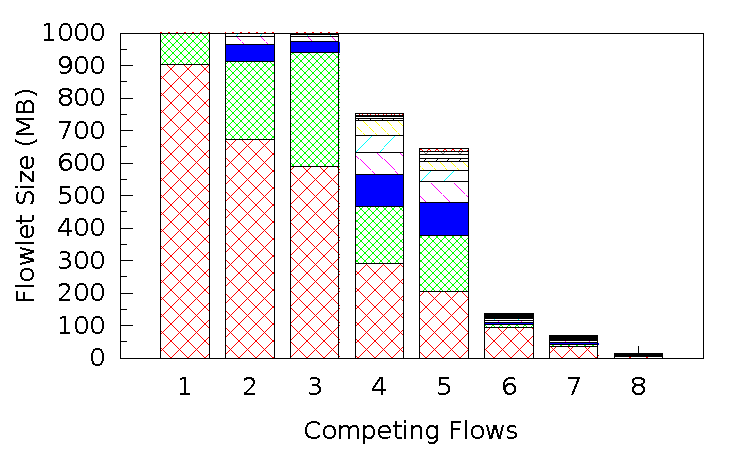
\includegraphics[width=0.45\textwidth]{./figures/flowlets/histo.pdf}
        \caption{Stacked histogram of flowlet sizes (in MB) for a 1 GB {\tt scp} file transfer. We vary the number of {\tt nuttcp}~\cite{nuttcp} background flows and
                denote them as {\em Competing Flows}. The size of each flowlet is shown within each bar, and flowlets
                are created whenever there is a 500 $\mu$s delay between segments. The top 10 flowlet sizes are shown here.
                We also analyzed the results of a 1 GB {\tt nuttcp}, {\tt ftp}, and a simple custom client/server transfer and found them
                to be similar. }
        \label{micro_flowlet_size}
\end{figure}

%\aditya{the following two paras don't flow well. they don't make a clear case for why flowlets is a bad idea and TSO segment level switching is a good idea. if reordering is the 100us flowlets' big problem then why not use our receiver-side reordering tricks with 100us flowlets? also it is not clear how were are overcoming reordering simply by relying on TSO segment switching}

%\eric{Rough estimates from our experiments with 100$\mu$s: ~90\% of flowlet sizes are 114KB or less with flowlets. ~00.1\% of flowlets are
%larger than 1 MB, with the largest ranging from 2.1-20.5MB. Some thoughts: (i) 100 $\mu$s flowlets can still have flowlet sizes larger 
%than switch buffers, which can cause congestion/loss when collision occur, (ii) given that flowlet with 100 $\mu$s does not prevent reordering,
%then why should we use flowlets at all? (iii) flowlets were really meant to have inactivity timers larger than the max difference in latency
%over any two paths, and buffer latency at one switch alone is ~4ms, so the use of flowlets on these small time scales is fundamentally
%flawed, (iv) flowlets are sensitive to traffic demand at sender, (v) flowlets are non-uniform in size, (vi) flowlets could break small 
%flows over multiple paths. Using TSO segment ensures: (i) small, uniform units of load-balancing, which means (ii) we are indenpendent
%of traffic demand, (iii) collisions are not a problem b/c TSO size is smaller than buffer size, (iv) most small flows are routed
%over the same path, (v) we do not impose too much computational overhead on sender/receiver and (vi) we still need to solve reordering.}

% Rough outline for next two paragraphs
% Problem with flowlets:
%  1. Sensitive to traffic patterns at the sender
%     a. In practice, we find this means the distribution of flowlet sizes is not uniform, and has a tail
%     b. These tails can still experience hash collisions, albeit less often.
%		i. congestion: lower throughput and to longer mice tail latencies
%  2. Needlessly break down small flows into several flowlets
%     a. Especially early in connection: 100us, 50 KB mice flows broken into 4-5 flowlets
%  3. Designed to be robust to reordering, but difficult to tune
%


Another possibility is to load balance on flowlets~\cite{conga,juniper-vcf}.  
A flow is comprised of a series of bursts, and a flowlet is created when
the inter-arrival time between two packets in a flow exceeds a threshold inactivity timer.  
In practice, inactivity timer values are between 100-500 $\mu$s~\cite{conga}. 
These values intend to strike a good balance between load balancing on a sub-flow level 
and acting as a buffer to limit reordering between flowlets.
Flowlets are derived from traffic patterns at the sender, and in practice this
means the distribution of flowlet sizes is not uniform. To analyze flowlet sizes, a simple experiment is shown in Figure~\ref{micro_flowlet_size}. 
We connect a sender and a receiver to a single switch and start an {\tt scp} transfer designed to 
emulate an elephant flow. Meanwhile, other senders are hooked up to the same switch and
send to the same receiver. We vary the number of these competing flows and show a stacked histogram of 
the top 10 flowlet sizes for a 1 GB {\tt scp} transfer with a 500 $\mu$s inactivity timer. 
The graph shows flowlet sizes can be quite large, with more than half the transfer being attributed
to a single flowlet for up to 3 competing flows. Using a smaller inactivity timer, such 100$\mu$s, helps (90\% of flowlet sizes are 114KB or less), but
does not prevent a long tail: 0.1\% of flowlets are larger than 1 MB, with the largest ranging from 2.1-20.5 MB.
Collisions on large flowlet sizes can lead to congestion.
The second problem with flowlets is that small inactivity thresholds, such as 100 $\mu$s, can lead to significant reordering.
Not only does this impact TCP performance (profiled in Section~\ref{sec:micro}), but it also needlessly 
breaks small flows into several flowlets. With only one flow in the network, we found a 50 KB
mice flow was broken into 4-5 flowlets on average. Small flows typically do not need to be
load balanced on a sub-flow level and need not be exposed to reordering.


%Another possibility is to load balance on flowlets~\cite{conga,juniper-vcf}.  A flow is typically comprised of a series of bursts, and each burst is defined as a flowlet. By monitoring the inter-arrival time of packets in a flow, one can easily define an inactivity timer to seperate flowlets.  In practice, intactivity timer values are between 100-500 $\mu$s~\cite{conga}. These values are intended to strike a good balance between creating enough opportunities to load balance on a sub-flow level and also ensure the reordering is limited at the destination due to the time buffer naturally incurred between flowlets.  We find, however, that it is difficult to strike a balance between achieving fine-grained, near-optimal load balancing and robustness against reordering. We perform a simple experiment in Figure~\ref{micro_flowlet_size}.  We connect a sender and a receiver to a single switch and start a transfer over an application designed to emulate an elephant flow ({\tt scp}). Meanwhile, we also hook up other senders to the same switch and have them send to the same reciever. We vary the number of competing flows and show a stacked histogram of the top 10 flowlet sizes for a 1 GB scp transfer with a 500 $\mu$s inactivity timer. \eric{Competing flows use nuttcp.} The graph shows flowlet sizes can be large, which means hash collisions can still occur on large flowlets.  Using a smaller timeout, such as 100 $\mu$s, creates smaller flowlets, but as we show in Section XXX, suffers from severe reordering that greatly reduces throughput and hurts applications.  \eric{mention creates congestion, which leads to lower thorughput and increase mice FCT latency}

% What do we want in sub-flow load balancing?
%  A. Want to move toward idealized ECMP: uniform sub-flow load balancing without the tail
%  B. Units should be as small as possible for fine-grained load balancing, but
%       not so small to be inefficient (TSO) or break small flows into parts
%  C. Independent of traffic patterns on sender
%  As a result, we settle on...

The shortcomings of the previous approaches lead us to reconsider on what granularity
load balancing should occur. 
%We take motivation from a best-case ECMP scenario. 
Ideally, sub-flow load balancing should be done on near uniform sizes.
%independent of traffic patterns on the sender to avoid long tails. 
Also, the unit of load balancing should be small to
allow for fine-grained load balancing, but not so small as to break small flows into 
many pieces or as to be a significant computational burden. As a result, we
propose load balancing on 64 KB units of data we call {\em flowcells}. Flowcells
have a number of advantages. First, the maximum segment size supported by TSO
is 64 KB, so flowcells provide a natural interface to high speed optimizations provided
by the NIC and OS and can scale to fast networking speeds. Second, an overwhelming fraction of mice flows are less than 64 KB in size
 and thus do not have to worry about reordering~\cite{benson10,vl2,kandula2009nature}.
Last, since most bytes in datacenter networks originate from elephant flows~\cite{kandula2009nature,benson10,dctcp},
this ensures that a significant portion of datacenter traffic is routed on uniform
sizes. While promising, this approach must combat reordering to be effective. 
Essentially we make a trade-off: 
%we provide line rate load balancing in the most effective
%manner as to avoid congestion and then handle reordering head-on at the receiver.
the sender avoids congestion by providing fine-grained, near-uniform load balancing,
and the receiver handles reordering to maintain line-rate.


%We highlight the challenges of this approach
%in the next subsection and provide a design to mitigate reordering problems in Section~\ref{sec:design}.

%In order to obtain fine-grained, near-optimal load balancing, we should stripe on a granularity
%that is indendpent of traffic patterns, near-uniform in size, and as small as possible while still
%scaling to fast network speeds.
%Therefore, we argue the TSO segment~\keqiang{what about saying maximum TSO segment size (64KB), each TSO segment's size is bounded by maximum TSO size} 
%is the natural granularity in which to load balance. Doing so
%provides several benefits. First, TSO segments are small and near-uniform in size, so an
%effective load-balancing scheme should be able to closely track the optimal case of per-packet
%load balancing, but without the additional computational overhead.
%Second, the TSO engine in the NIC will ensure that all packets created from a TSO segment will contain the same
%header information. We show in Section XXX how this is important to deal with reordering because
%we can easily impart metadata on all packets within a segment that help us distinguish loss from 
%ordering~\keqiang{all the packets within the same flowcell contain the same flowcell id.  
%"all packets created from a TSO segment will contain the same
%header information" is fine but a flowcell can contrain several TSO segments depending on TSO segment size}.
%Last, small flows less than 64 KB in size will actually be routed over the
%same path in the network, meaning a very large fraction of mice flows will not be routed on a subflow
%level and thus do not have to worry about reordering~\cite{benson10,vl2,kandula2009nature}~\keqiang{Around 90\% of datacenter flows' sizes are smaller than 64KB~\cite{benson10}, 
%meaning the overwhelming majority is load balanced like ECMP and we only need to engineering the left 10\%}.
%\eric{need to mention that we can combine segments as long as not above 64 KB, so not really
%per TSO segment. helps in small flows.}
%While promising, this approach has a major challenge: reordering. We highlight these challenges
%in the next subsection and provide a design to mitigate the problems in Section~\ref{sec:design}.

\tightparagraph{Per-Hop vs End-to-End Multipathing}
The last design consideration is whether multipathing should be done on a local, per-hop level (\eg{}, ECMP), or
on a global, end-to-end level. In Presto, we choose the latter: pre-configured end-to-end paths
are allocated in the network and path selection (and thus multipathing) is realized by having the network edge
place flowcells onto these paths. 
Presto can be used to load-balance in an ECMP style per-hop manner, but the choice of end-to-end 
multipathing provides additional benefits due to greater control of how flowcells are mapped to
paths. Per-hop multipathing can be inefficient
under asymmetric topologies~\cite{wcmp}, and load-balancing on a global end-to-end level can allow
for weighted scheduling at the vSwitch to rebalance traffic. This is especially important when failure occurs.
The second benefit is flowcells can be assigned over multiple paths very evenly
by iterating over paths in a round-robin, rather than randomized, fashion. 

%As we show
%in Section~\ref{sec:micro}, randomization in per-hop multipathing can lead to "unluckiness" where
%multiple flowcells get sent to the same link over a small timescale by multiple flows. This transient congestion
%can lead to increased buffer occupancy and higher delays in the network. These benefits can
%fundamentally be provided at the per-hop level (\cite{wcmp} handles asymmetry), but require changes to networking firmware. 
%These considerations motivate us to utilize end-to-end multipathing, but Presto can also
%use per-hop multipathing when conveinent.

\subsection{Reordering Challenges}
%The above design decisions in Presto cause following main challenges:
Due to the impact of fine-grained, flowcell-based load balancing, Presto must account for reordering. Here, we 
highlight reordering challenges. The next section shows how Presto deals with these concerns.

%\tightparagraph{Soft Edge Distributed Load Balancing}
%There are two main challenges in implementing load balancing at the soft edge. First, the implementation
%must scale to fast networking speeds because networking at 10+ Gbps can have significant overhead if not carefully
%considered. Therefore, in order to achieve line rate, great care must be taken to ensure that load balancing
%schemes are light-weight, simple and can take advantage of optimizations provided by the NIC and OS.  
%The second major problem is how to load balance in a distributed fashion at the vSwitches in such
%a way that the load balancing performs well globally.
%Nodes must ensure they are spreading
%their traffic equally throughout the network, but in a low-overhead fashion that does not require detailed
%topographical information about the network, real-time traffic matrices, or strict coordination
%with other senders.

%\eric{several things to add: in presto, we can just make dumb edge decisions and not have to worry
%about (i) the traffic patterns, that is who else is sending, (ii) topology asymmetry. Basically,
%we want to highight that the vSwitch shouldn't require a lot of detailed network-wide information,
%but should be able to somehow still load balance in a way that performs very well globally.}

\tightparagraph{Reordering's Impact on TCP} The impact of reordering on TCP is well-studied~\cite{leung2007overview,paxson1997end}. 
Duplicate acknowledgments caused by reordering
can cause TCP to move to a more conservative sender state and reduce the sender's congestion window.
Relying on parameter tuning, such as adjusting the DUP-ACK threshold, is not ideal because 
increasing the DUP-ACK threshold increases the time to recover from real loss. Other TCP settings
such as Forward Acknowledgement (FACK) assume un-acked bytes in the SACK are lost and degrade
performance under reordering. 
A scheme that introduces reordering should not rely on careful configuration of TCP parameters
because (i) it is hard to find a single set of parameters that work effectively over multiple 
scenarios and (ii) datacenter tenants should not be forced to constantly tune their networking stacks.
Finally, many reordering-robust variants of TCP have been proposed~\cite{rr-tcp,blanton2002making,tcp-pr}, but
as we will show, GRO becomes ineffective under reordering. Therefore, reordering should
be handled below the transport layer.

\tightparagraph{Computational Bottleneck of Reordering}
Akin to TSO, Generic Receive Offload (GRO) mitigates the computational burden of receiving
1500 byte packets at 10 Gbps. GRO is implemented in the kernel of the hypervisor,
and its handler is called directly by the NIC driver. It is responsible
for aggregating packets into larger segments that are pushed up to OVS and the TCP/IP stack. 
GRO is implemented in the Linux kernel and is used even without virtualization. Similar
functionality can be found in Windows (RSC~\cite{ms-rsc}) and hardware (LRO~\cite{grossman2005large}).

Because modern CPUs use aggressive prefetching, the cost of receiving
TCP data is now dominated by per-packet, rather than per-byte, operations.
As shown by Menon~\cite{optimize-tcp-receive},  the majority of this overhead comes from
buffer management and other routines not related to protocol processing, and therefore 
significant computational overhead can be avoided by aggregating "raw" packets from
the NIC into a single {\tt sk\_buff}.
%\footnote{Refer to~\cite{linuxgro,optimize-tcp-receive} for detailed study and explanation}
Essentially, spending a few cycles to aggregate packets within GRO creates less segments for
TCP and prevents having to use substantially more cycles at higher layers in the networking stack.
Refer to~\cite{linuxgro,optimize-tcp-receive} for detailed study and explanation.

To better understand the problems reordering causes, a brief description of  
the TCP receive chain in Linux follows. First, interrupt coalescing allows the NIC to create an interrupt for a batch of packets~\cite{mogul1997eliminating,understanding-linux-network},
which prompts the driver to poll the packets into an aggregation queue. Next, the driver
invokes the GRO handler, located in the kernel, which
{\em merges} the packets into larger segments. The merging continues,
possibly across many polling events, until a segment
reaches a threshold size, a certain age, or cannot be combined with the incoming packet. Then, the
combined, larger segment is {\em pushed up} to the rest of the TCP/IP networking stack. The GRO process is
done on a per-flow level. With GRO disabled, throughput drops to around
5.7-7.1 Gbps and CPU utilization spikes to 100\% (Section~\ref{sec:micro} and~\cite{bullettrains}). 
Receive offload algorithms, whether in hardware (LRO)~\cite{grossman2005large,open-lro} or in software (GRO), are usually
{\em stateless} to make them fast: no state is kept beyond the segment being merged.


%\begin{figure}[!htb]
%        \centering
%  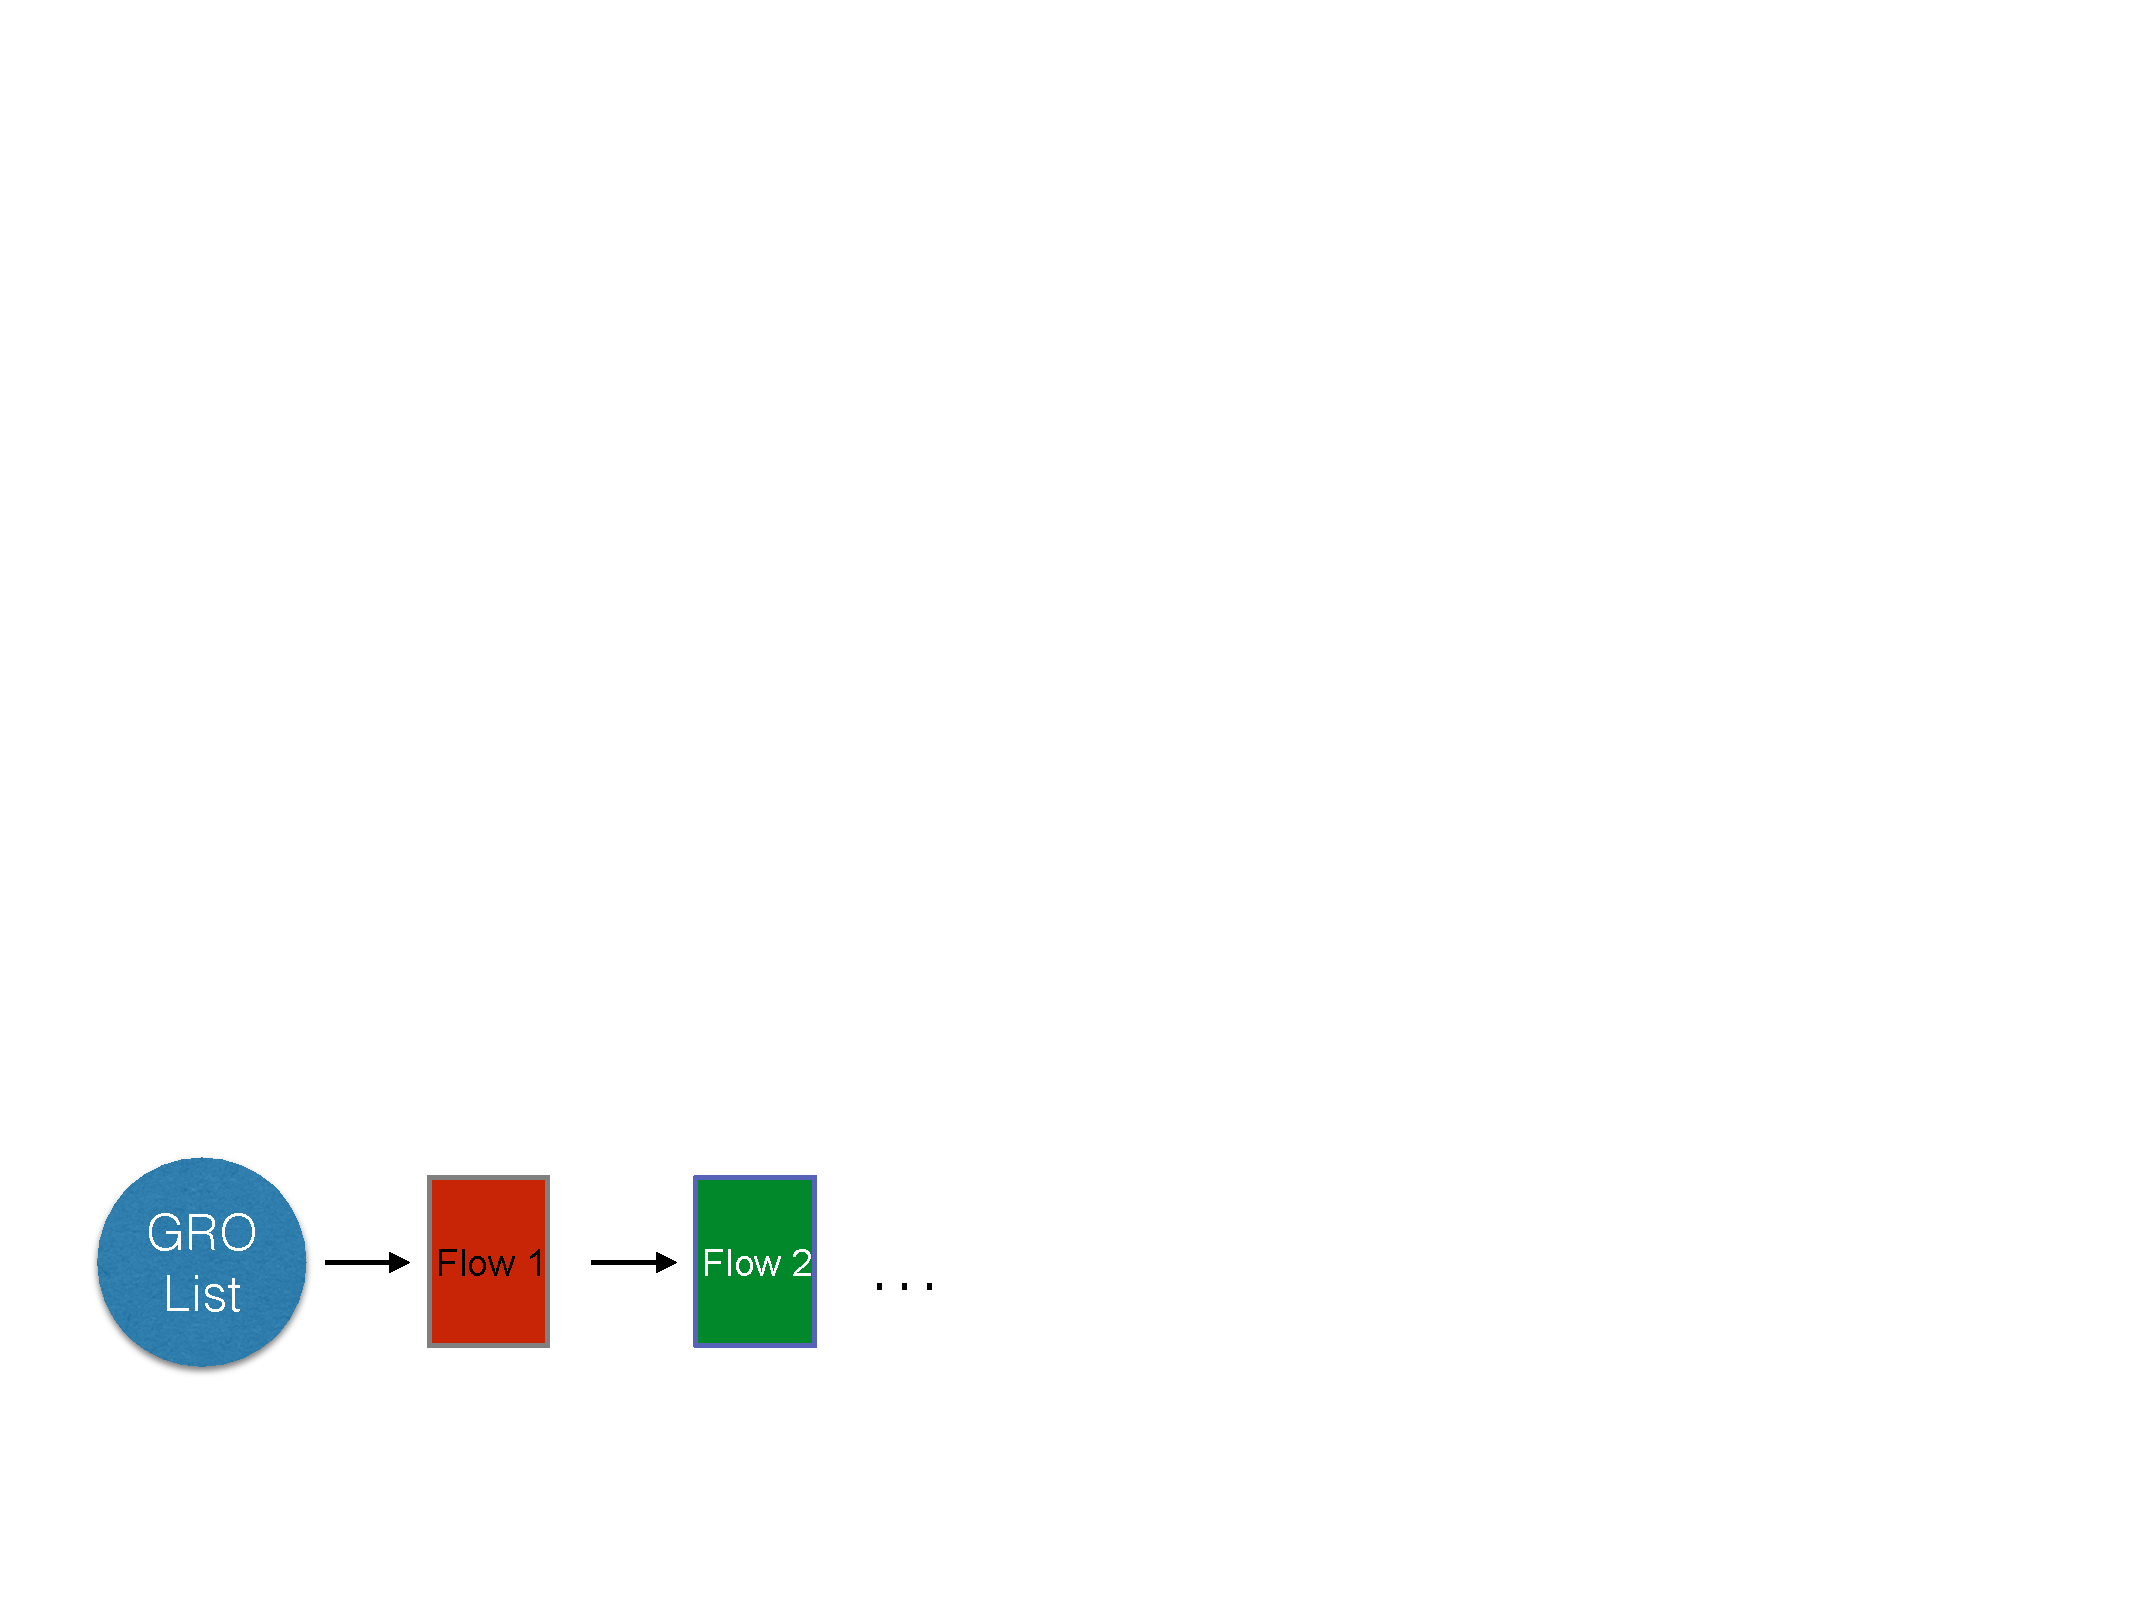
\includegraphics[width=0.45\textwidth]{./figures/gro-design/gro.pdf}
%        \caption{GRO design. FIX ME!}
%        \label{gro-design}
%\end{figure}

\begin{figure}[t]
        \centering
  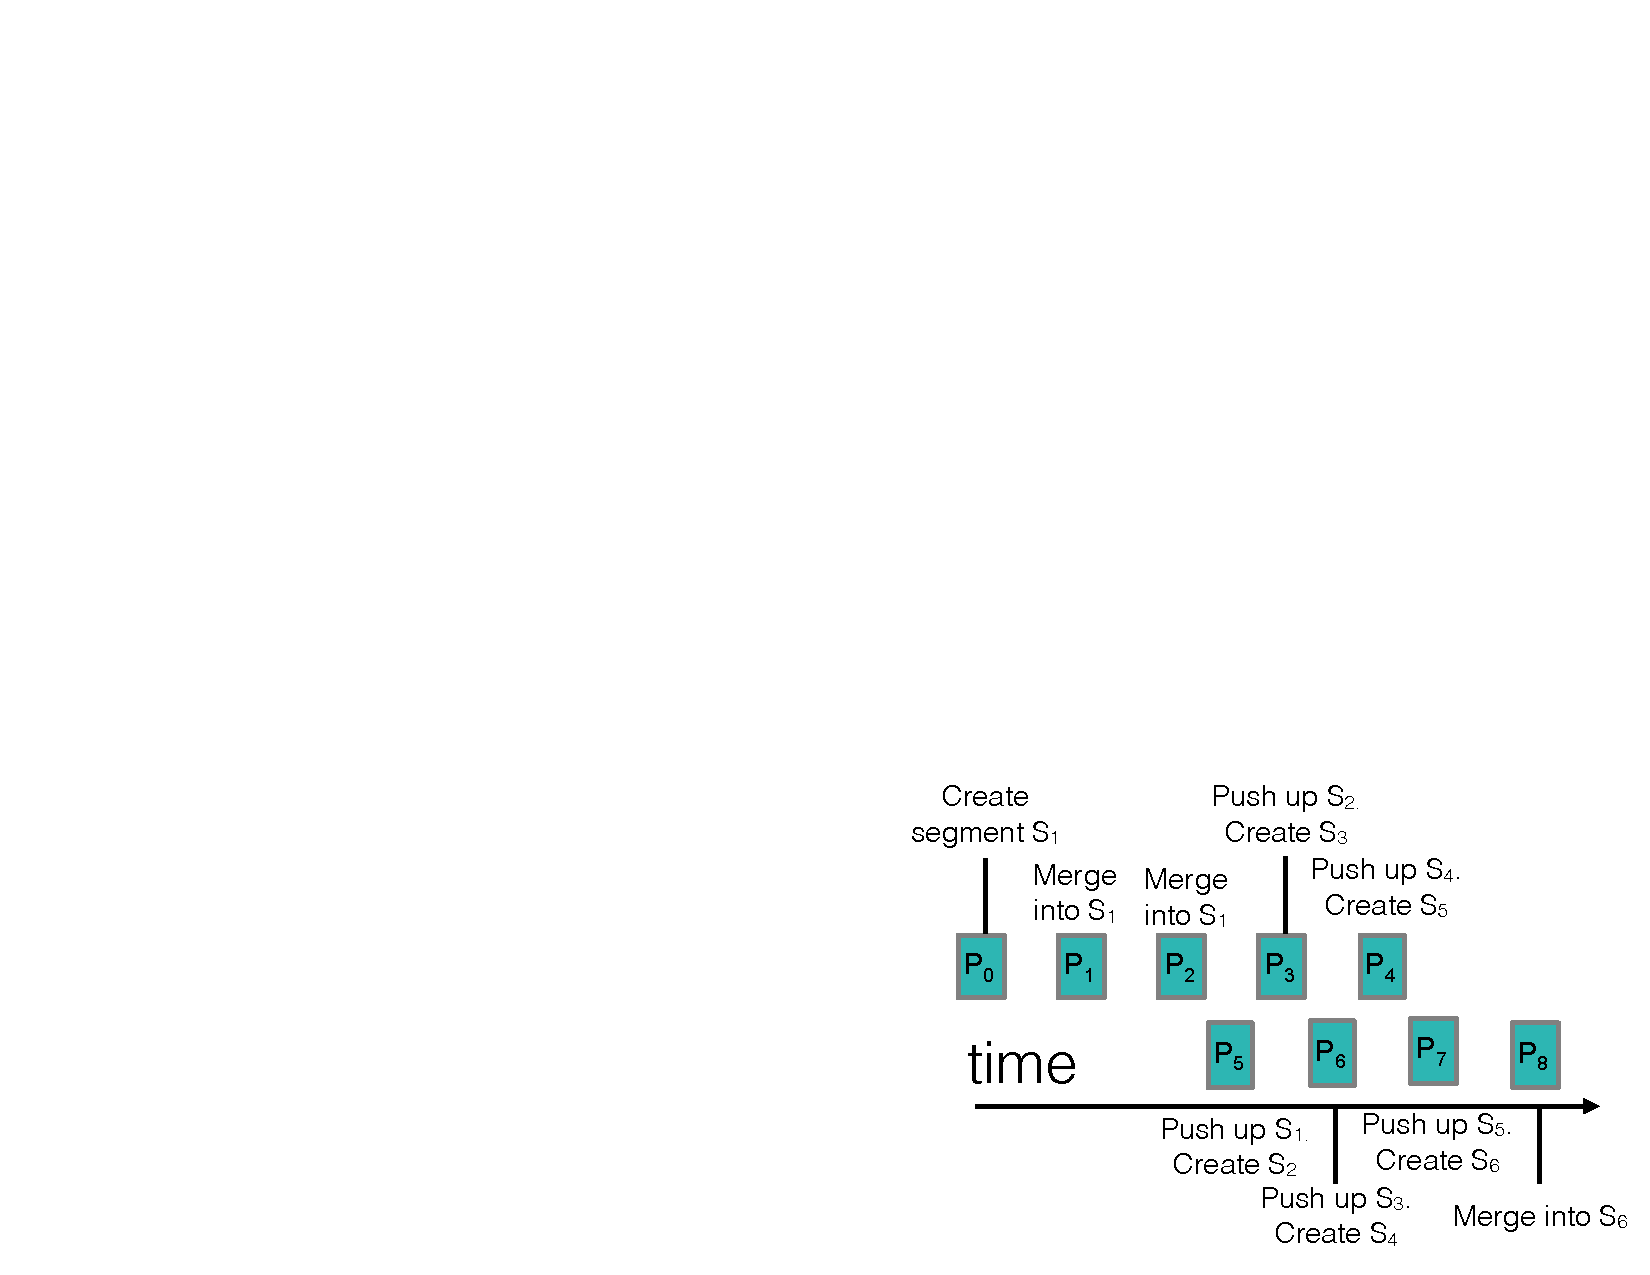
\includegraphics[width=0.45\textwidth]{./figures/gro-design/gro-break.pdf}
        \caption{GRO pushes up small segments ($S_i$) during reordering.}
        \label{gro-break}
\end{figure}


We now uncover how GRO breaks down in the face of reordering. Figure~\ref{gro-break} shows the impact of reordering on GRO.  Reordering does not allow the segment to grow: each reordered packet cannot be merged with the existing segment, and thus the previously created segment must be pushed up. With extreme reordering, GRO is effectively disabled because small MTU-sized segments are constantly pushed up. This causes (i) severe computational overhead and (ii) TCP to be exposed to significant amounts of reordering. We term this the {\em small segment flooding} problem.

Determining where to combat the reordering problem has not previously taken the small segment flooding problem into account.  Using a reordering buffer to deal with reordered packets is a common solution (\eg{}, works like~\cite{drb} re-sort out-of-order packets in a shim layer below TCP), but a buffer implemented above GRO cannot prevent small segment flooding.  Implementing a buffer below GRO means that the NIC must be changed, which is (i) expensive and cumbersome to update and (ii) unlikely to help combat reordering over multiple interrupts.

In our system, the buffer is implemented in the GRO layer itself.  We argue this is a natural location because GRO can
directly control segment sizes while simultaneously limiting the impact of reordering. 
Furthermore, GRO can still be applied on packets pushed up from LRO, which means hardware doesn't have to be modified
or made complex.
Implementing a better GRO algorithm has multiple challenges. The algorithm should be light-weight to scale to fast networking speeds. Furthermore, an ideal scheme should be able to distinguish loss from reordering.  When a gap in sequence numbers is detected (\eg{}, when $P_5$ is received after $P_2$ in Figure~\ref{gro-break}), it is not obvious if this gap is caused from loss or reordering.  If the gap is due to reordering, GRO should not push segments up in order to try to wait to receive the missing gap and merge the missing packets into a preestablished segment.  If the gap is due to loss, however, then GRO should immediately push up the segments to allow TCP to react to the loss as fast as possible. Ideally, an updated GRO algorithm should ensure TCP does not perform any worse than a scheme with no reordering. Finally, the scheme should adapt to prevailing network conditions, traffic patterns and application demands.




\section{Design}
\label{design}
\begin{figure}[!t]
        \centering
  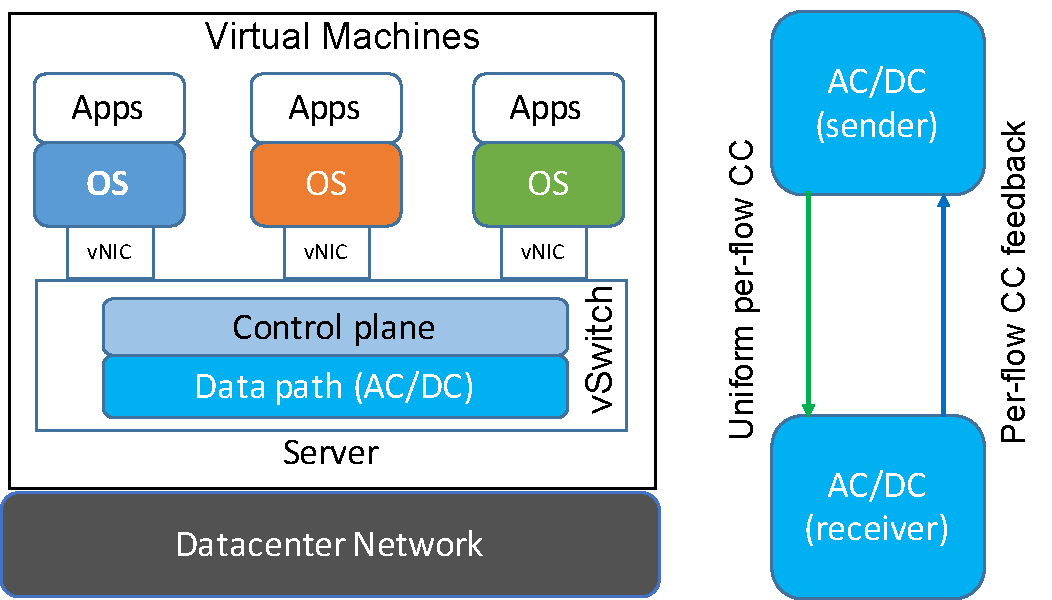
\includegraphics[width=0.45\textwidth]{figures/acdc_highlevel.pdf}
        \caption{\acdc{} high-level architecture.}
        \label{acdc_highlevel}
\end{figure}

This section provides an overview of~\acdc{}'s design. First, we show how basic
congestion control state can be inferred in the vSwitch. Then we study
how to implement DCTCP. Finally, we discuss how to enforce congestion
control in the vSwitch and provide a brief overview of how per-flow differentiation
can be implemented.


\begin{figure}[th]
        \centering
  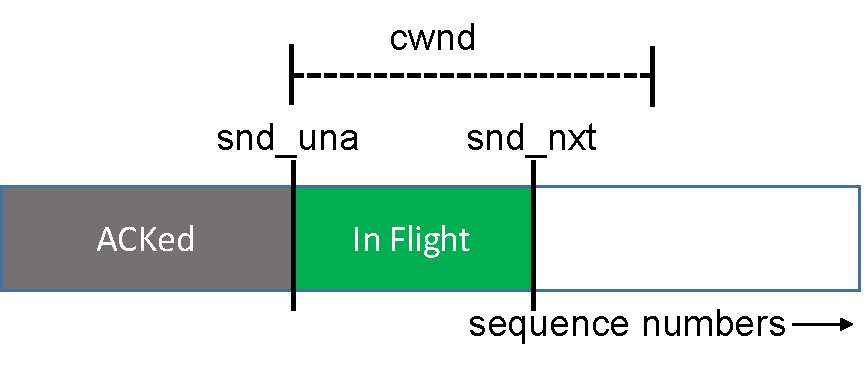
\includegraphics[width=0.45\textwidth]{figures/tcp-state-new.pdf}
        \caption{Variables for TCP sequence number space.}
        \label{tcpstate}
\end{figure}
\subsection{Obtaining Congestion Control State}
\label{ss:tcpstate}
Figure~\ref{acdc_highlevel} shows the high-level structure of \acdc{}. Since it is
implemented in the datapath of the vSwitch, all traffic can be monitored. The sender
and receiver modules work together to implement per-flow congestion control (CC).

We first demonstrate how congestion control state can be inferred.
Figure~\ref{tcpstate} provides a visual of the TCP sequence number space. The {\tt snd\_una} variable is the first byte
that has been sent, but not yet ACKed. The {\tt snd\_nxt} variable is the 
next byte to be sent. Bytes between {\tt snd\_una} and {\tt snd\_nxt} are in flight.
The largest number of packets that can be sent and unacknowledged is bounded by \cwnd{}.
{\tt snd\_una} is simple to update: each ACK contains an acknowledgement number ({\tt ack\_seq}), and 
{\tt snd\_una} is updated when {\tt ack\_seq} $>$ {\tt snd\_una}.
When packets traverse the vSwitch from the VM, {\tt snd\_nxt} is updated if the sequence
number is larger than the current {\tt snd\_nxt} value.
Detecting loss is also relatively simple. If {\tt ack\_seq $\le$ snd\_una}, then
a local {\tt dupack} counter is updated. Timeouts can be inferred when {\tt snd\_una $<$ snd\_nxt}
and an inactivity timer fires. The initial~\cwnd{} is set to a default value of 10~\cite{RFC6928}. 
With this state, the vSwitch can determine appropriate~\cwnd{} values for canonical
TCP congestion control schemes.
%More advanced congestion control techniques that rely on timestamps, round-trip times, SACKs or 
%FACKs can also be implemented. 
We omit additional details in the interest of space. 



\subsection{Implementing DCTCP}
%\begin{figure}[!t]
%        \centering
%  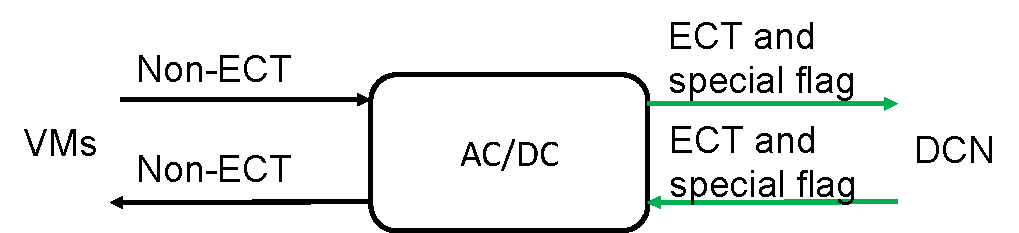
\includegraphics[width=0.45\textwidth]{figures/acdc_ECT_marking.pdf}
%        \caption{Simple stateless ECT marking in \acdc{}. 
%		Turn all intra-DC TCP packets in the fabric into ECT.}
%        \label{acdc_ect_marking}
%\end{figure}

%\begin{figure}[!t]
%        \centering
%  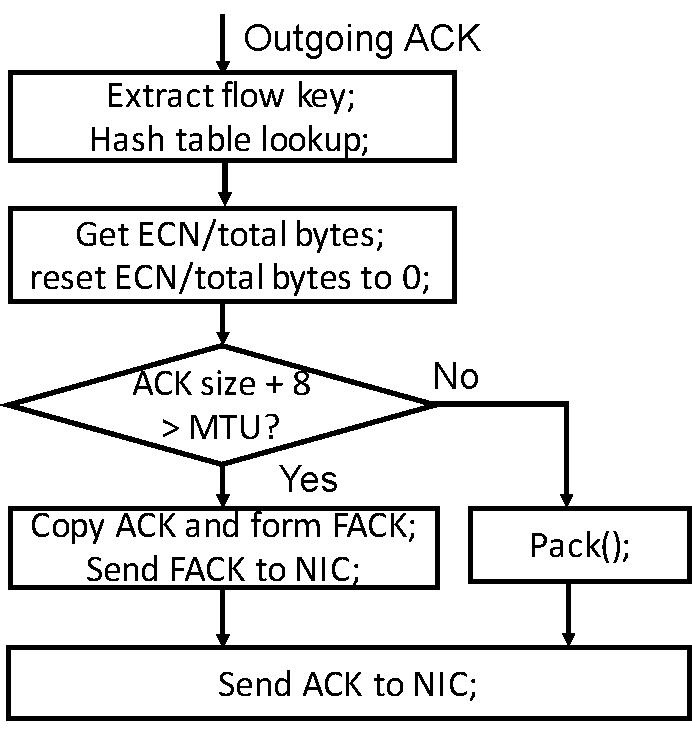
\includegraphics[width=0.25\textwidth]{figures/carry_ecn_info.pdf}
%        \caption{Carrying the congestion information back. 
%		Being compatible with TSO and minimizing CPU and traffic overhead.}
%        \label{acdc_carry_ecn_info}
%\end{figure}

This section discusses how to obtain DCTCP state and perform its congestion control.


\tightparagraph{ECN marking} 
DCTCP requires flows to be ECN-capable, but the VM's TCP stack may not support ECN.
Thus, all egress packets are marked to be ECN-capable on the sender module. 
When the VM's TCP stack does not support ECN, all ECN-related bits on ingress packets are stripped at the sender
and receiver modules in order to preserve the original TCP settings. When the VM's TCP
stack does support ECN, the~\acdc{} modules strip the {\tt congestion encountered} 
bits in order to prevent the VM's TCP stack from decreasing rates too aggressively
(recall DCTCP adjusts~\cwnd{} proportional to the fraction of congested packets, while traditional schemes conservatively reduce~\cwnd{} by half). A reserved bit in
the header is used to determine if the VM's TCP stack originally 
supported ECN.
%Algorithm~\ref{alg:non-ect-to-ect} changes non-ECT packets into ECT packets
%in the virtual switch before the packets enter the fabric and
%change them back when they arrive at the destination virtual switch.
%$p.pretendECT$ is set or cleared by flipping the 2nd bit of the 3 reserved bits in TCP header.
%After applying this algorithm, all TCP packets traversing the network appear to be ECT packets.
%So the ECT and non-ECT coexistence issue is solved.
%Also, because we change non-ECT back at the destination virtual switch,
%so TCP is not aware of such a transformation and \acdc{} does not break any TCP connections or applications.
%Algorithm~\ref{alg:non-ect-to-ect} leverages hardware checksumming feature in the NIC implicitly to reduce CPU overhead.
%\todo{how to add comment in this algorithm?}.
%
%
%\begin{algorithm}[t]
%\caption{ECT marking in \acdc{}}
%\label{alg:non-ect-to-ect}
%\begin{algorithmic}[1]
%%\STATE \Comment{packet $p$ is TCP packet}
%\IF{$p$ is going to the network}
%\IF{$p$ is non-ECT}
%\STATE change $p$ to ECT by modifying IP header
%\STATE set $p.pretendECT$
%%\STATE set the 2nd bit of the 3 reserved bits in TCP header to 1
%\ENDIF
%\ELSIF{$p$ is coming from the network}
%\IF{$p$ is non-ECT and $p.pretendECT$ is set}
%\STATE change $p$ back to non-ECT by modifying IP header
%\STATE clear $p.pretendECT$
%%\STATE clear the 2nd bit of the reserved bits
%\ENDIF
%\ENDIF
%\end{algorithmic}
%\end{algorithm}
%

\tightparagraph{Obtaining ECN feedback}
In DCTCP, the fraction of packets experiencing congestion needs to be reported to the sender. 
%DCTCP relays this information from the destination to the sender by essentially modulating data
%in the ACK reporting scheme. Sender and receiver agree on an ACK state-machine that effectively 
%communicates how many packets were received with ECN vs how many were not. Because the TCP stack
%in the VM may not be DCTCP, we do not want to rely on the ACK modulation scheme. 
Since the VM's TCP stack may not support ECN, the~\acdc{} receiver module monitors
the total and ECN-marked bytes received for a flow. Receivers piggy-back the
reported totals on ACKs by adding an additional 8 bytes as a TCP Option. This is called 
a Piggy-backed ACK (PACK). The PACK is created by moving the IP and TCP headers into
the ACK packet's {\tt skb} headroom~\cite{kernel-skb}. The totals are inserted into the vacated space and the memory
consumed by the rest of the packet (\ie{}, the payload) is left as is. The IP header checksum, IP packet length and TCP Data Offset fields are recomputed and the 
TCP checksum is calculated by the NIC. The PACK option is stripped at the
sender so it is not exposed to the VM's TCP stack. 

If adding a PACK creates a packet larger than the MTU, the NIC offload feature (\ie{}, TSO)
will replicate the feedback information over multiple packets, which skews the feedback.
Therefore, a dedicated feedback packet called a Fake ACK (FACK) is sent when the MTU
will be violated. The FACK is sent in addition to the real TCP ACK.
FACKs are also discarded by the sender after logging the included
data. In practice, most feedback takes the form of PACKs.

%
%\begin{algorithm}[t]
%\caption{Carrying the congestion information back}
%\label{alg:outgoing}
%\begin{algorithmic}[1]
%%\STATE flow\_key $\leftarrow$ \{dstip, srcip, dstport, srcport\}
%%\STATE ack\_entry $\leftarrow$ rcv\_ack\_hashtbl\_lookup(flow\_key)
%%\STATE end\_seq $\leftarrow$ ntohl(tcp.seq) + tcp.data\_len
%%\IF{after(end\_seq, ack\_entry.snd\_nxt)}
%%       \STATE ack\_entry.snd\_nxt $\leftarrow$ end\_seq
%%\ENDIF
%%\IF{tcp.ack}
%\IF{outgoing skb is a TCP ACK}
%\STATE flow\_key $\leftarrow$ \{dstip, srcip, dstport, srcport\}
%\STATE entry $\leftarrow$ rcv\_data\_hashtbl\_lookup(flow\_key)
%        \IF{entry.total\_bytes > 0}
%                \STATE ecn\_bytes $\leftarrow$ entry.ecn\_bytes
%                \STATE total\_bytes $\leftarrow$ entry.total\_bytes
%                \STATE entry.ecn\_bytes $\leftarrow$ 0
%                \STATE entry.total\_bytes $\leftarrow$ 0
%        \ENDIF
%        \IF{total\_bytes > 0}
%                \IF{skb.data\_len < (MTU -- HEADROOM)}
%                        \STATE skb $\leftarrow$ ovs\_pack(skb, ecn\_bytes, total\_bytes)
%                \ELSE
%                        \STATE fack $\leftarrow$ ovs\_fack(skb, ecn\_bytes, total\_bytes)
%                \ENDIF
%        \ENDIF
%\ENDIF
%\IF{fack != NULL}
%        \STATE sendtoNIC(fack)
%\ENDIF
%\STATE sendtoNIC(skb)
%\end{algorithmic}
%\end{algorithm}
%

\begin{figure}[!t]
        \centering
  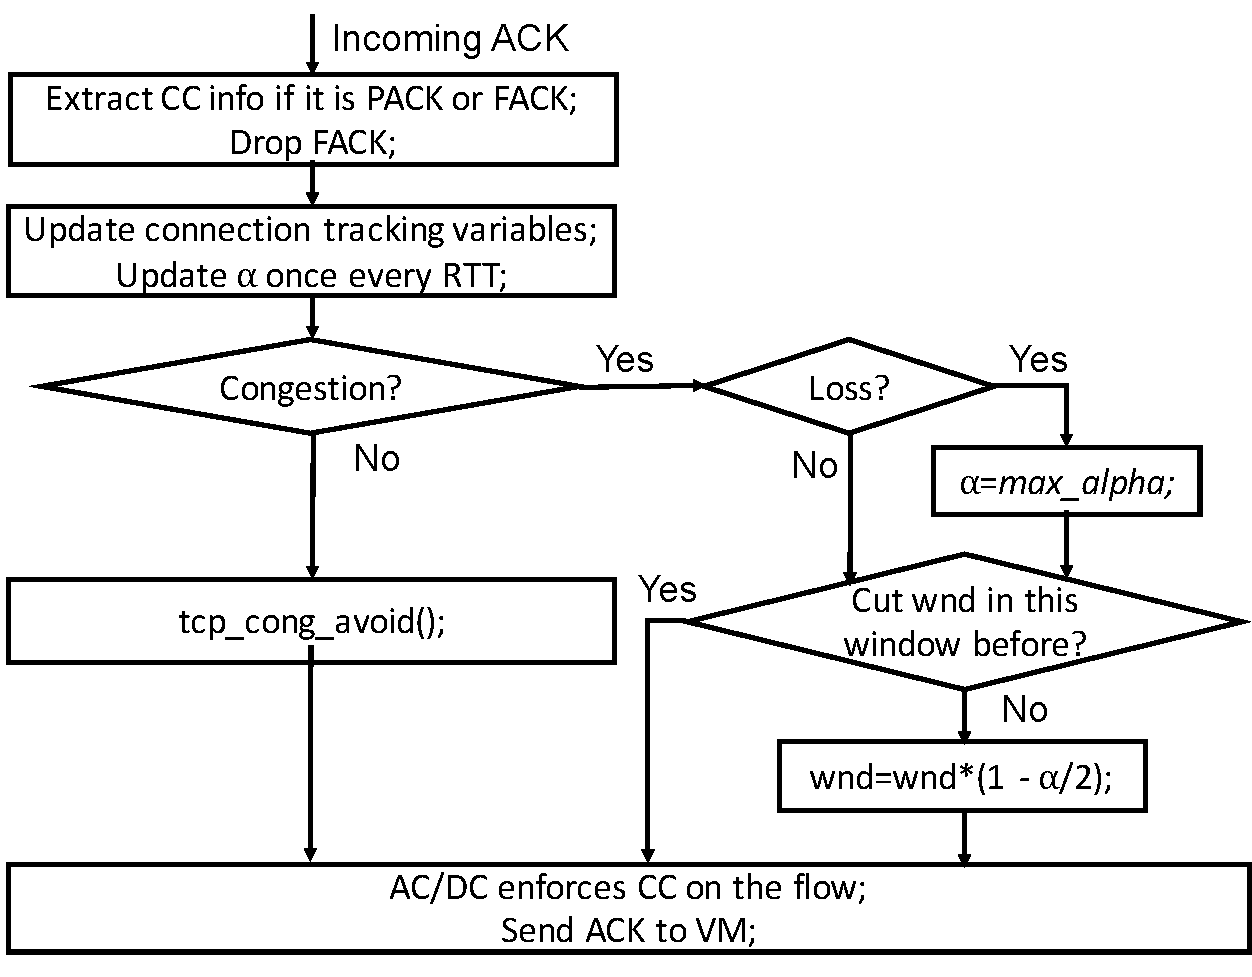
\includegraphics[width=0.49\textwidth]{figures/acdc_cc.pdf}
        \caption{DCTCP congestion control in \acdc{}.}
        \label{acdc_cc}
\end{figure}
\tightparagraph{DCTCP congestion control} 
Once the fraction of ECN-marked packets is obtained, implementing DCTCP's logic is straightforward.
Figure~\ref{acdc_cc} shows the high-level design. 
First, congestion control (CC) information is extracted from FACKs and PACKs. Connection tracking
variables (described in \cref{ss:tcpstate}) are updated based on the ACK. The variable
$\alpha$ is an EWMA of the fraction of packets that experienced congestion and is updated roughly
once per RTT. If congestion was not encountered (no loss or ECN), then {\tt tcp\_cong\_avoid} advances~\cwnd{}
based on TCP New Reno's algorithm, using slow start or congestion avoidance as needed. If congestion was
experienced, then~\cwnd{} must be reduced. DCTCP's instructions indicate the window should
be cut at most once per RTT.
Our implementation closely tracks the Linux source code, and
additional details can be referenced externally~\cite{alizadeh2011data,ietf-tcpm-dctcp}.


%\begin{algorithm}[!tbh]
%\caption{Congestion control in \acdc{}}
%\label{alg:incoming}
%\begin{algorithmic}[1]
%\IF{incoming skb is a TCP ACK}
%\STATE initialize is\_rack, is\_pack and is\_fack
%\STATE flow\_key $\leftarrow$ \{srcip, dstip, srcport, dstport\}
%\STATE entry $\leftarrow$ rcv\_ack\_hashtbl\_lookup(flow\_key)
%\IF{is\_pack or is\_fack}
%        \STATE unpack and extract ecn\_bytes and total\_bytes
%        \STATE update(entry.ecn\_bytes, ecn\_bytes)
%        \STATE update(entry.total\_bytes, total\_bytes)
%\ENDIF
%\IF{is\_rack or is\_pack}
%        \STATE acked $\leftarrow$ tcp.ack\_seq -- entry.snd\_una
%        \STATE entry.snd\_una $\leftarrow$ tcp.ack\_seq
%        \IF{duplicated ACK}
%                \STATE entry.dupack\_cnt++
%        \ENDIF
%        \STATE dctcp\_update\_alpha(entry)
%        \IF{acked > 0}
%                \IF{may\_raise\_rwnd(entry)}
%                        \STATE tcp\_cong\_avoid(entry, acked)
%                \ENDIF
%        \ENDIF
%\ENDIF
%\IF{entry.dupack\_cnt >= 3 or ecn\_bytes > 0}
%        \IF{entry.dupack\_cnt >= 3}
%                \STATE entry.alpha $\leftarrow$ MAX\_ALPHA
%                \STATE entry.loss $\leftarrow$ true
%        \ENDIF
%        \IF{may\_reduce\_rwnd(entry)}
%                \STATE entry.ssthresh $\leftarrow$ dctcp\_ssthresh(ack\_entry)
%                \STATE entry.rwnd $\leftarrow$ min(RWND\_MIN, entry.ssthresh)
%                \STATE entry.reduced $\leftarrow$ true
%        \ENDIF
%\ENDIF
%\IF{is\_rack or is\_pack}
%        \STATE tcp.window $\leftarrow$ min(tcp.window, entry.rwnd)
%\ENDIF
%\IF{is\_fack}
%        \STATE drop(skb)
%\ENDIF
%\ENDIF
%\end{algorithmic}
%\end{algorithm}
%

\subsection{Enforcing Congestion Control}
\label{ss:enforce}
There must be a mechanism to ensure a VM's TCP flow adheres to the~\cwnd{} determined in the vSwitch.
Luckily, TCP provides built-in functionality that can be reprovisioned for~\acdc{}. Specifically,
TCP's flow control allows a receiver to advertise the amount of data it is willing to process via
a receive window (\rwnd{}).~\crs{Similar to other works~\cite{Kalampoukas02,Spring00}, the vSwitch overwrites~\rwnd{} with its calculated~\cwnd{}}.
In order to preserve TCP semantics, this value is overwritten only when it is smaller than the packet's original~\rwnd{}.
The VM's flow then uses $min(\cwnd{},\rwnd{})$ to limit how many packets it can send.

This enforcement scheme must be compatible with TCP receive window scaling to work in practice.
Scaling ensures~\rwnd{} does not become an unnecessary upper-bound in high bandwidth-delay networks
and provides a mechanism to left-shift~\rwnd by a window scaling factor~\cite{RFC1323}. 
The window scaling factor is negotiated during TCP's handshake, so~\acdc{} monitors handshakes
to obtain this value. Calculated congestion windows are adjusted accordingly.
TCP receive window auto-tuning~\cite{semke1998automatic} manages buffer state
and thus is an orthogonal scheme~\acdc{} can safely ignore.

Ensuring a VM's flow adheres to~\rwnd{} is relatively simple. The vSwitch calculates a new congestion 
window every time an ACK is received. This value provides a bound on the number of bytes the VM's flow
is now able to send. VMs with unaltered TCP stacks will naturally follow our enforcement scheme because the stacks
will simply follow the standard. Flows that circumvent the standard can be policed by dropping
excess packets not allowed by the calculated congestion window, which incentivizes tenants to respect the standard.

While simple, this scheme provides a surprising amount of flexibility. For example, TCP enables
a receiver to send a TCP Window Update to update~\rwnd{}~\cite{RFC5681}.~\acdc{}
can create these packets to update windows without relying on ACKs.
Additionally, the sender module can generate duplicate ACKs to to trigger retransmissions. This is useful when 
the VM's TCP stack has a larger timeout value than~\acdc{} (\eg{}, small timeout values
have been recommended for incast~\cite{vasudevan2009safe}). 
%In this case, the vSwitch can send three dup-ACKs (with
%an appropiate~\rwnd{}) to trigger the VM's TCP flow to retransmit.
% EJR-- put back in for camera ready?
\crs{
Another useful feature is when~\acdc{} allows a TCP stack to send {\em more} data. This can occur when
a VM TCP flow aggressively reduces its window when ECN feedback is received. By removing ECN feedback
in~\acdc{}, the VM TCP stack won't reduce~\cwnd{}. 
In a similar manner, DCTCP limits loss more effectively than aggressive TCP stacks. Without loss
or ECN feedback, VM TCP stacks grow~\cwnd{}. This causes~\acdc{}'s~\rwnd{} to become the limiting window, and thus~\acdc{} can 
increase a flow's rate instantly when~\rwnd{} $<$ \cwnd{}. Note, however,~\acdc{} cannot force
a connection to send more data than the VM's~\cwnd{} allows.
}

Another benefit of~\acdc{} is that it scales in the number of flows.
Traditional software-based rate limiting schemes, like Linux's Hierarchical Token Bucket, 
incur high overhead due to frequent interrupts and contention~\cite{radhakrishnan2014senic} and
therefore do not scale gracefully. NIC or switch-based rate limiters are low-overhead, but typically
only provide a handful of queues. Our enforcement algorithm does not rate limit or buffer packets because it exploits TCP
flow control. Therefore, rate limiting schemes can be used at a coarser granularity (\eg{}, VM-level).


~\crs{
Finally, we outline~\acdc{}'s limitations. 
Since~\acdc{} relies on sniffing traffic, schemes that encrypt TCP headers (\eg{}, IPSec) are not supported. Our implementation only supports TCP, but we believe it can be extended to handle UDP similar to
prior schemes~\cite{shieh2011sharing,jeyakumar2013eyeq}.
Implementing per-flow DCTCP-friendly UDP tunnels and studying its impact remains future work, however. And finally, 
while MPTCP supports per-subflow~\rwnd{}~\cite{RFC6824}, it is not included in our case study and a more detailed analysis
is future work.
}
 


%\tightparagraph{Compatible with receive window auto-tuning and window scaling}
%TCP receive window auto-tuning~\cite{semke1998automatic,receive-auto-runing} is a commonly used feature 
%in modern TCP stacks. It is enabled by default in recent Linux and Windows distributions.
%Receive window auto-tuning was proposed to automatically 
%set socket buffer size based on network conditions to 
%improve network performance while optimizing the memory usage by TCP connections.
%Because \acdc{} overwrites the real \rwnd{} value embedded in TCP ACK header 
%only when \acdc{}'s running \rwnd{} is smaller than 
%the real \rwnd{}, thus \acdc{} does not break the correctness of TCP semantics 
%and is compatible with receive window auto-tuning.
%

\begin{figure}[t]
        \centering
        \begin{subfigure}[b]{0.225\textwidth}
                \centering
                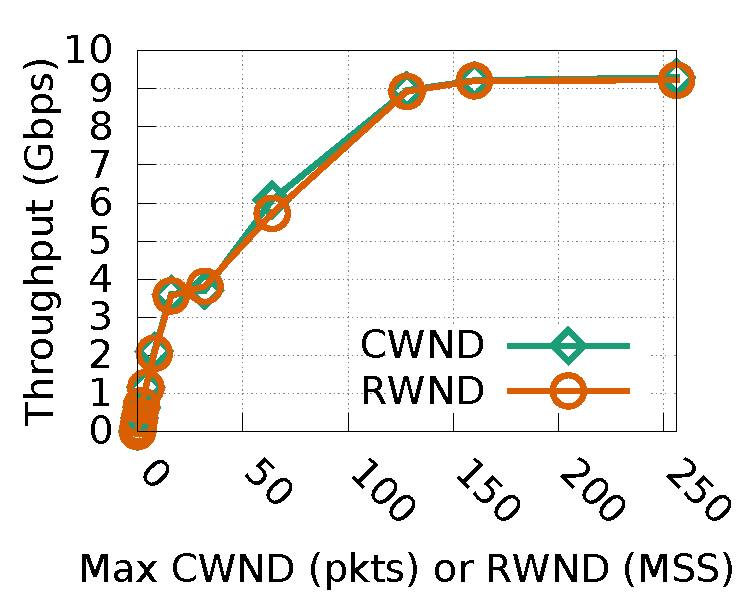
\includegraphics[width=\textwidth]{figures/new_enforce/new_tput_cwnd_rwnd_cubic_15k.pdf}
                \caption{MTU = 1.5KB.}
                \label{effectiveness_15k}
        \end{subfigure}
        \begin{subfigure}[b]{0.225\textwidth}
                \centering
                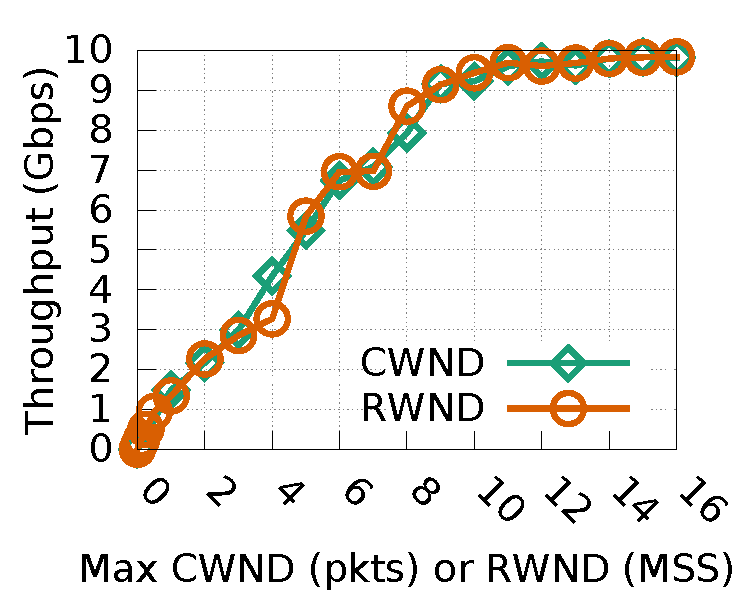
\includegraphics[width=\textwidth]{figures/new_enforce/new_tput_cwnd_rwnd_cubic_9k.pdf}
                \caption{MTU = 9KB.}
                \label{effectiveness_9k}
        \end{subfigure}
        \caption{Using \rwnd{} can effectively control throughput.}
                %Experiments are conducted on a 10G testbed. TCP CUBIC but New Reno shows similar results.
                %Linux 3.18.0. We control maximal \rwnd{} value by modifying the receiver's advertised window size in TCP ACKs
                %in the Open vSwitch. We control maximal \cwnd{} by specifying ``snd\_cwnd\_clamp" value in Linux TCP.}
        \label{rwnd_effectiveness}
\end{figure}
\subsection{Per-flow Differentiation}
\label{ss:cc-qos}
\acdc{} can assign different congestion control algorithms
on a per-flow basis. This gives administrators additional flexibility and control by 
assigning flows to specific congestion control algorithms based on policy.
For example, flows destined to the WAN may be assigned CUBIC and flows destined within the
datacenter may be set to DCTCP. 

Administrators can also enable per-flow bandwidth allocation schemes.
A simple scheme enforces an upper-bound
on a flow's bandwidth. Traditionally, an upper-bound on a flow's~\cwnd{} can be
specified by {\tt snd\_cwnd\_clamp} in Linux.~\acdc{} can provide similar functionality
by bounding~\rwnd{}. Figure~\ref{rwnd_effectiveness} shows the behavior is equivalent. This 
graph can also be used to convert a desired upper-bound on bandwidth into an appropriate maximum~\rwnd{} (the
graph is created on an uncongested link to provide a lower bound on RTT). 

In a similar fashion, administrators can assign different bandwidth priorities to flows by altering the 
congestion control algorithm. Providing differentiated services via congestion control has 
been studied~\cite{Venkataramani2002tcpnice,shieh2011sharing}. Such schemes are useful because networks
typically contain only a limited number of service classes and bandwidth may need to be allocated on
a finer-granularity. We propose a unique priority-based congestion control algorithm for~\acdc{}.
Specifically, DCTCP's congestion control algorithm is modified to incorporate a priority, $\beta \in [0,1]$:
\begin{equation}
rwnd = rwnd (1 - (\alpha - \frac{\alpha{}\beta}{2}))
\label{eqn:cc-qos}
\end{equation}
Higher values of $\beta$ give higher priority. 
When $\beta{}=1$, Equation~\ref{eqn:cc-qos} simply converts to DCTCP congestion control. When
$\beta{}=0$, flows aggressively back-off (\rwnd{} is bounded by 1 MSS to avoid starvation). This equation
alters multiplicative decrease instead of additive increase because increasing~\rwnd{} 
cannot guarantee the VM flow's~\cwnd{} will allow the flow to increase its sending rate.

%subsection{How to keep low overhead?}
%Move to Implementation?
%Connection tracking~\cite{ayuso2006netfilter,ovs-conntrack}.
%
%\subsection{How is it complimentary to other schemes?}
%Like bandwidth allocation.
%
%~\eric{Should we talk about how we can actually increase rate of VM TCP?}
%


%In history, TCP used packet loss as the signal of network congestion. 
%But, using packet loss as the signal can not meet the performance demand of datacenter environment 
%due to high queueing latency and frequent packet losses. Packet loss-based congestion control 
%can work reasonably well for large data transfers but does harm time-critical RPCs. 
%Thus, new congestion control algorithms designed for datacenter networks were proposed. 
%They can be classified into 2 categories: Explicit Congestion Notification (ECN)-based and 
%latency-based. The most straightforward way is to treat ECN as packet loss and cut congestion 
%window before network queue built up and packet loss happens---but this can harm flow throughput. 
%DCTCP improves this by cut window properly based on the portion of marked packets and 
%gives high throughput for large flows and low latency for mice flows. 
%Latency-based congestion control such as TCP-NV, TIMELY, DX use the end-to-end latency 
%as the signal of network congestion. Compared with ECN-based approach, latency is a more 
%prevalent signal for congestion (i.e., does not need ECN capability on the switches). 
%But the challenge of such approaches is to find ways to combat with latency measurement noise 
%caused by TSO, LRO and interrupt coalescence.
%


%\begin{figure}[t]
%        \centering
%        \begin{subfigure}[b]{0.225\textwidth}
%                \centering
%                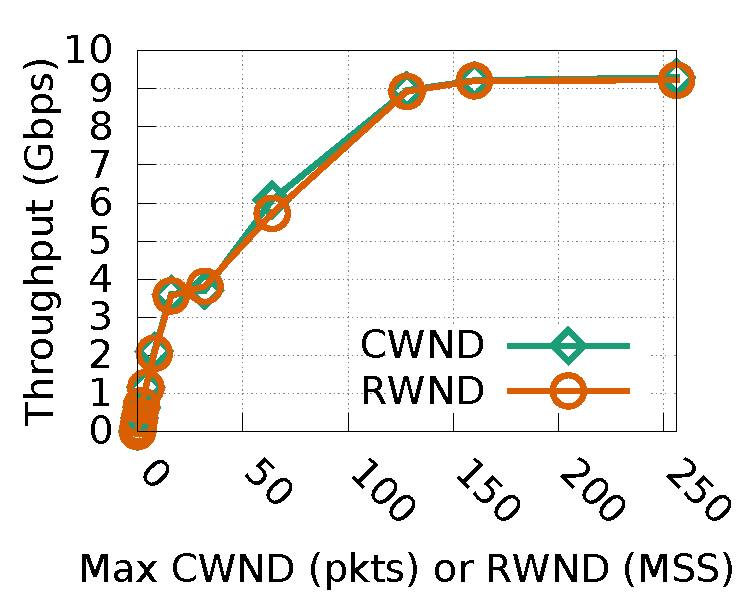
\includegraphics[width=\textwidth]{figures/new_enforce/new_tput_cwnd_rwnd_cubic_15k.pdf}
%                \caption{MTU = 1.5KB.}
%                \label{effectiveness_15k}
%        \end{subfigure}
%        \begin{subfigure}[b]{0.225\textwidth}
%                \centering
%                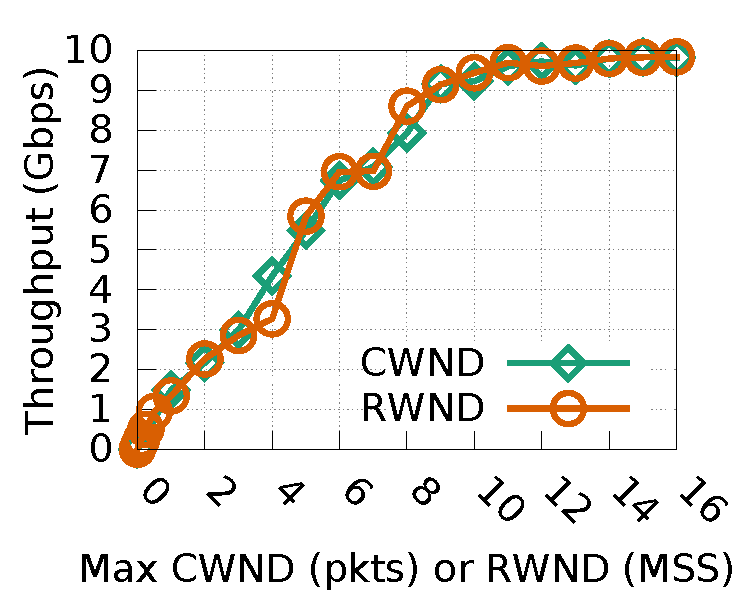
\includegraphics[width=\textwidth]{figures/new_enforce/new_tput_cwnd_rwnd_cubic_9k.pdf}
%                \caption{MTU = 9KB.}
%                \label{effectiveness_9k}
%        \end{subfigure}
%        \caption{Using \rwnd{} can effectively control throughput. 
%		Experiments are conducted on a 10G testbed. TCP CUBIC but New Reno shows similar results.
%		Linux 3.18.0. We control maximal \rwnd{} value by modifying the receiver's advertised window size in TCP ACKs
%		in the Open vSwitch. We control maximal \cwnd{} by specifying ``snd\_cwnd\_clamp" value in Linux TCP.}
%        \label{rwnd_effectiveness}
%\end{figure}

\section{Implementation}
\label{impl}
This section outlines relevant implementation details. We
implemented~\acdc{} in Open vSwitch (OVS) v2.3.2~\cite{ovs-website} and
added about 1200 lines of code (many are debug/comments). 
A high-level overview follows.
\crs{
A hash table is added to OVS, and flows are hashed on a 5-tuple (IP addresses, ports and VLAN) to obtain a flow's state.
The flow entry state is 320 bytes and is used to maintain the congestion control state mentioned in \cref{design}.
SYN packets are used to create flow entries, and FIN packets, coupled with a course-grained garbage
collector, are used to remove flow entries. Other TCP packets, such as data and ACKs, trigger 
updates to flow entries.
There are many more table lookup operations (to update flow state)
than table insertions or deletions (to add/remove flows). Thus, Read-Copy-Update (RCU)
hash tables~\cite{guniguntala2008read} are used to enable efficient lookups.
Additionally, individual {{\tt spinlocks}} are used on each flow entry in order to allow
for multiple flow entries to be updated simultaneously.
}

\crs{
Putting it together, the high-level operation on a data packet is as follows. An application on the sender generates a packet
that is pushed down the network stack to OVS. The packet is intercepted in {\tt  ovs\_dp\_process\_packet}, where the
packet's flow entry is obtained from the hash table. Sequence number state is updated in the flow entry and ECN bits are set on
the packet if needed (see \cref{design}).
If the packet's header changes, the IP checksum is recalculated. Note TCP checksumming is offloaded to the NIC.
The packet is sent over the wire and received at the receiver's OVS. The receiver updates congestion-related state, strips
off ECN bits, recomputes the IP checksum, and pushes the packet up the stack. ACKs eventually triggered by the packet
are intercepted, where the congestion information is added. Once the ACK reaches the sender, the~\acdc{} module uses
the congestion information to compute a new congestion window. Then it modifies~\rwnd{} with a {{\tt memcpy}}, 
strips off ECN feedback and recomputes the IP checksum before pushing the packet up the stack.
Since TCP connections are bi-directional, two flow entries are maintained for each connection. 
}

\crs{
Our experiments in~\cref{micro} show the CPU overhead of~\acdc{} is small and several implementation details
help reduce computational overhead. First, OVS sits 
above NIC offloading features (\ie{}, TSO and GRO/LRO) in the networking stack. Briefly, NIC offloads allow 
the host to pass large data segments along the TCP/IP stack and only deal with MTU-sized packets in the NIC. Thus,~\acdc{}
operates on a segment, rather than a per-packet, basis. Second, 
congestion control is a relatively simple algorithm, and thus the computational burden is not high. Finally,
while~\acdc{} is implemented in software, it may be possible to further reduce the
overhead with a NIC implementation. Today, "smart-NICs"
implement OVS-offload functionality~\cite{cavium-nic,netronome-nic},  
naturally providing a mechanism to reduce overhead and support hypervisor bypass (\eg{}, SR-IOV). 
}
%We have also considered designing an~\acdc{}-enabled middlebox to support
%legacy systems that do not run OVS and cannot upgrade their NICs.


%
%Standard OVS kernel datapath LoC: 2360
%\acdc{} kernel datapath LoC: 3590
%
%\tightparagraph{UDP traffic} How to handle.
%Mention VxLAN traffic too.
%\keqiang{and IPsec}
%
%\tightparagraph{No vSwitch}
%\keqiang{title should be hypervisor-bypass?}
%Use middleboxes (for DB server).
%Use NIC (for SR-IOV).
%Hypervisor bypass (e.g., SR-IOV), where TCP traffic is sent to the NIC directly without
%going through hypervisor. First, as noted by~\cite{shieh2011sharing}, ``loss of the security and
%manageability features provided by the software virtual switch has limited
%the deployment of direct I/O NICs in public clouds''. Second, based on techniques like Intel
%DPDK~\cite{intel-dpdk} and ``smart NICs''~\cite{cavium-nic,netronome-nic}, we believe that low latency
%congestion control enforcement schemes like \acdc{} can also be
%employed for hypervisor bypass use cases.
%We need to worry about legacy systems and non-VM systems. For instance, a database or storage device that may not have OVS installed on it.
%We need to talk about either a middlebox or that this percentage of traffic is low? Or implement in NIC (especially one with OVS offload?).
%
%
%\tightparagraph{Little CPU and memory overhead}
%In our implementation, first we leverage the Read-Copy-Update (RCU)~\cite{guniguntala2008read} enabled hash tables
%to keep per-flow states (such as ``snd\_una'' and ``snd\_nxt''). RCU technique is also employed by
%Open vSwitch's kernel datapath and it helps improve processing speed for ``read-heavy''
%workloads (\ie{}, inserting new flows is much less frequent than looking-up existing flows) on
%shared-memory multiprocessor systems.
%Second, \acdc{} processes on ``segment'' level instead of ``packet'' level due to
%NIC offloading features (TSO at the sender side and GRO/LRO at the receiver side).
%Third, we also leverage the NIC checksumming offloading feature such that
%we do not need to compute checksums after we change TCP/IP header fields.
%Our microbenchmarks (\cref{micro}) show that \acdc{} incurs very little additional CPU overhead (less than 4\%) to
%support 10Gbps line-rate, even it is fully implemented in software.
%We are currently implementing \acdc{} on Cavium's programmable NICs~\cite{cavium-nic},
%where we can entirely offload the computational overhead to hardware. Therefore, we believe
%\acdc{} can support even higher line rates (\eg{}, 40Gbps).
%In our implementation, each TCP connection takes 320 bytes in the hash tables,
%so it takes around 3.2MB even there are 10K concurrent connections.
%{~\keqiang{i think we may want to mention that we use both FACK and PACK because we want to be compatible with TSO and try to minimize the CPU/traffic overhead.}

\section{Results}
\label{results}
This section quantifies
the effects of~\acdc{} and determines if the performance of DCTCP
implemented in the vSwitch (\ie{}, \acdc{}) is equivalent to
the performance of DCTCP implemented in the host TCP stack.

\tightparagraph{Testbed}
The experiments are conducted on a physical testbed with 17 
IBM System x3620 M3 servers (6-core Intel Xeon
2.53GHz CPUs, 60GB memory) and Mellanox ConnectX-2 EN 10GbE NICs.
Our switches are IBM G8264 (Broadcom Trident+), each with a buffer of 9MB shared
by forty-eight 10G ports and four 40G ports.
The switches have dynamic memory management enabled by default.

\tightparagraph{System settings}
We run Linux kernel 3.18.0 which implements DCTCP as a 
pluggable module~\cite{linux-dctcp}.
We set {{\tt $RTO_{min}$} to 10 ms~\cite{vasudevan2009safe,judd2015nsdi} and
configured the MTU to 9kB (unless otherwise noted).
We also set {\tt tcp\_low\_latency}, {\tt tcp\_no\_metrics\_save}, {\tt tcp\_sack} to 1 and
keep other parameters as default.


\tightparagraph{Experiment details}
To understand the performance of~\acdc{}, three different congestion control configurations
are considered. The baseline scheme, referred to as {\em CUBIC}, configures
the host TCP stack as CUBIC (Linux's default congestion control), which runs on top of an unmodified version of OVS.
Our goal is to be similar to {\em DCTCP}, which configures the host TCP
stack as DCTCP and runs on top of an unmodified version of OVS. Our scheme,{\em ~\acdc{}},
configures the host TCP stack as CUBIC (unless otherwise stated) and implements DCTCP congestion control in OVS.
In DCTCP and~\acdc{}, WRED/ECN is configured on the switches. In CUBIC,
WRED/ECN is not configured.

The performance metrics used are: TCP RTT (measured by sockperf~\cite{sockperf}),
TCP throughput (measured by iperf),
packet loss rate (by collecting switch counters) and
Jain's fairness index~\cite{jain-index}.
In \cref{macro}, flow completion time (FCT)~\cite{dukkipati2006flow} is used 
to quantify application-level performance.

\section{Microbenchmarks}
\label{sec:micro}

We first evaluate the effectiveness of Presto over a series of microbenchmarks: %. Using 
%canonical topologies, we investigate 
(i) Presto's effectiveness in preventing the small segment
flooding problem and reordering, (ii) Presto's CPU overhead, (iii) Presto's ability to scale
to multiple paths, (iv) Presto's ability to handle congestion, (v) comparison to flowlet
switching, and (vi) comparison to local, per-hop load balancing.

%%%%%micro test - scalability and congestion test topology
\begin{figure}[t]
        \centering
	\begin{subfigure}[b]{0.225\textwidth}
        	\centering
  		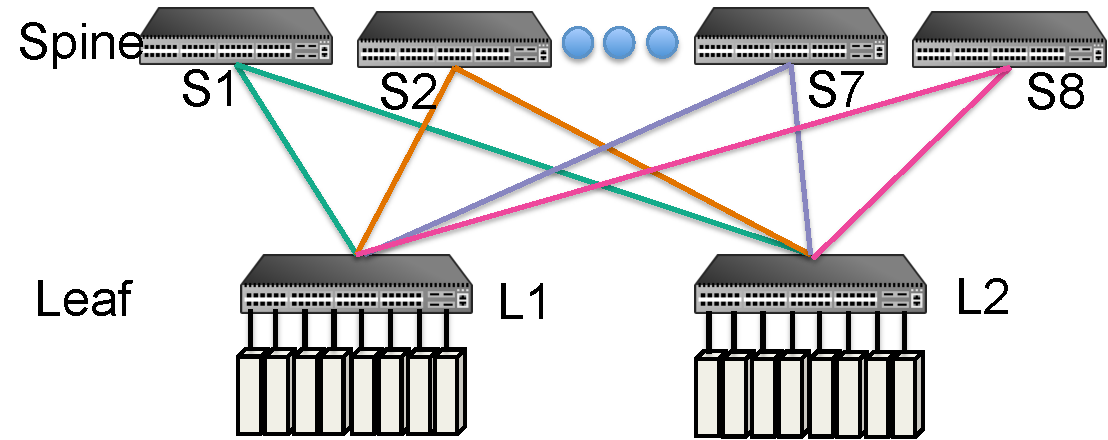
\includegraphics[width=\textwidth]{./figures/micro_test_topology/micro_scalabilitytest_topology_refined.pdf}
        	\caption{}
		\label{micro_scalability_topology}
	\end{subfigure}
	\begin{subfigure}[b]{0.225\textwidth}
                \centering
		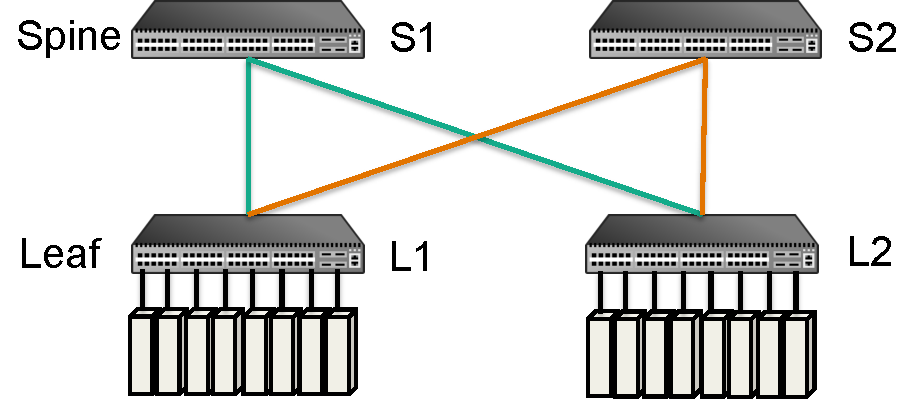
\includegraphics[width=\textwidth]{./figures/micro_test_topology/micro_congestiontest_topology_refined.pdf}
        	\caption{}
		\label{micro_congestion_topology}
	\end{subfigure}
	\caption{(a) Scalability benchmark and (b) Oversubscription benchmark topology.}
	\label{micro_topology}
\end{figure}

%%%%%gro effectiveness shows
\begin{figure}[t]
	\centering
	\begin{subfigure}[b]{0.225\textwidth}
                \centering
  		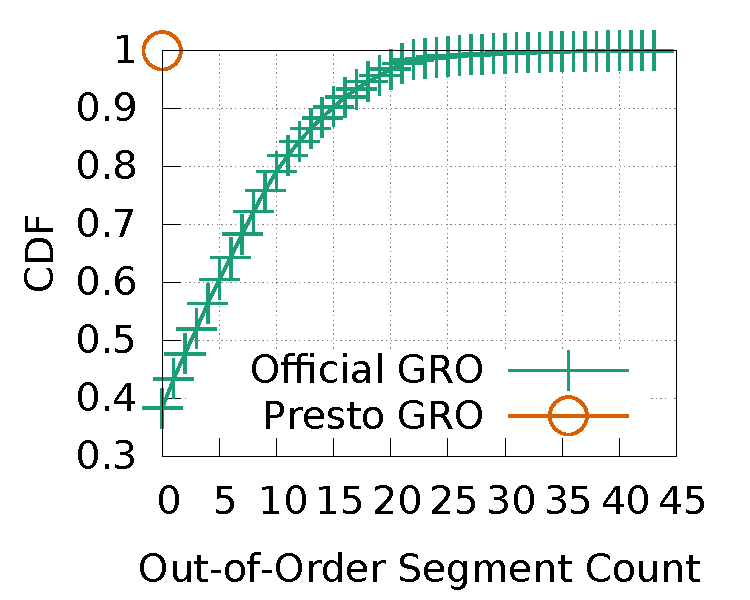
\includegraphics[width=\textwidth]{./figures/gro_effectiveness/metric1_seg_cdf_compare.pdf}
		\caption{}
		\label{gro_effectiveness_on_reordering}
	\end{subfigure}
        \begin{subfigure}[b]{0.225\textwidth}
                \centering
		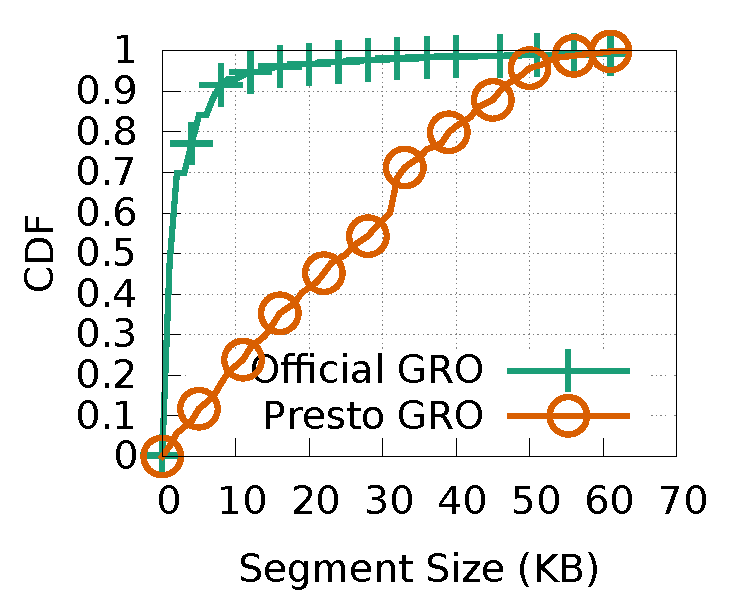
\includegraphics[width=\textwidth]{./figures/gro_effectiveness/metric1_pktsize_cdf_compare.pdf}
        	\caption{}
		\label{gro_effectiveness_on_pktsize}
	\end{subfigure}
	\caption{(a) Illustration of the modified GRO's effectiveness on masking reordering. 
		%We use the number of  segments from other chunks
                %between the first segment and last segment of each chunk
                %seen by TCP to measure the extent of packet reordering
		(b) In case of massive packet reordering, official GRO cannot merge packets effectively such that lots of small
                packets are processed by TCP which poses great processing overhead for CPU.}
	\label{gro_effectiveness}
\end{figure}

\tightparagraph{Presto's GRO Combats Reordering}
To examine Presto's ability to handle packet reordering, we perform a simple experiment
on the topology shown in Figure~\ref{micro_congestion_topology}.
%we compare the extent of TCP reordering, TCP segment size distribution, throughput and receiver side CPU usage 
%using official GRO and Presto GRO. 
Here two servers attached to leaf switch L1 
send traffic to their own receivers attached to leaf switch L2
by spreading flowcells over two network paths. 
%Because these two flows share the same two paths 
%so packet reordering can happen at the receiver side.
This setup can cause reordering for each flow, so 
we compare Presto's GRO to
an unmodified GRO, denoted "Official GRO". 
The amount of reordering exposed to TCP is presented in Figure~\ref{gro_effectiveness_on_reordering}.
To quantify packet reordering, we show a CDF of the {\em out-of-order segment count}: ~\ie{},
the number of segments from other flowcells between the first packet and last packet of each flowcell. A value of zero
means there is no reordering and larger values mean more reordering. The figure shows Presto's GRO can completely mask reordering
while official GRO incurs significant reordering. As shown in Section~\ref{sec:background}, reordering can
also cause smaller segments to be pushed up the networking stack, causing significant processing overhead.
Figure~\ref{gro_effectiveness_on_pktsize} shows the received TCP segment size distribution.  Presto's GRO
pushes up large segments, while the official GRO pushes up many small segments.
The average TCP throughputs in official GRO and Presto GRO are 4.6 Gbps (with 86\% CPU utilization) and 
9.3 Gbps (with 69\% CPU utilization), respectively. Despite the fact that official GRO only obtains 
about half the throughput of Presto's GRO, it still incurs more than 24\% higher CPU overhead. 
Therefore, an effective scheme must deal with both reordering and small segment overhead.
%\eric{interesting that stride on big testbed w/ official GRO had same numbers: 4.6 Gbps and similar overhead}

\begin{figure}[t]
        \centering
  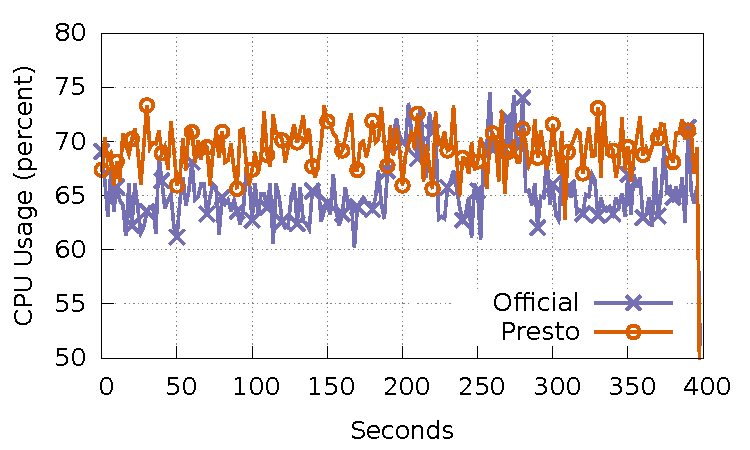
\includegraphics[width=0.45\textwidth]{./figures/mornitor_cpu/macro_compare_cpu_usage.pdf}
        \caption{Presto incurs 6\% CPU overhead on average.}
        \label{micro_compare_cpu}
\end{figure}

\tightparagraph{Presto Imposes Limited CPU Overhead}
We investigate Presto's CPU usage by
running the stride workload on a 2-tier Clos network as shown in Figure~\ref{macro_evaluation_topology}. 
For comparison, official GRO is run with the stride workload using a non-blocking switch (so there
is no reordering). Note both official GRO and Presto GRO can achieve 9.3 Gbps.  
The receiver CPU usage is sampled every 2 seconds over a 400 second interval, and
the time-series is shown in Figure~\ref{micro_compare_cpu}. 
%implying that the network utilization is 93% in both cases. 
On average, Presto GRO only increases CPU usage by 6\% compared with the official GRO. 
The minimal CPU overhead comes from Presto's careful design and implementation. 
At the sender, Presto needs just two {\tt memcpy} operations (1 for shadow MAC rewriting, 1 for flowcell ID encoding). 
At the receiver, Presto needs one {\tt memcpy} to rewrite the shadow MAC back to the real MAC and
also incurs slight overhead because multiple segments are now kept per flow. The overhead
of the latter is reduced because these segments are largely kept in reverse sorted order, which means {\tt merge}
on an incoming packet is usually $\mathcal{O}(1)$. The insertion sort is done at the beginning of each {\tt flush} event over a small
number of mostly in-order segments, which amortizes overhead because it is called infrequently compared to {\tt merge}.

%%%%%scalability test figures %%%%
\begin{figure}[t]
        \centering
  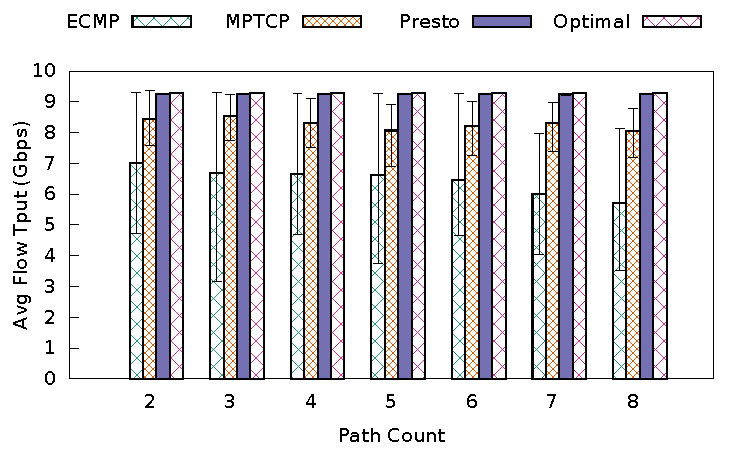
\includegraphics[width=0.45\textwidth]{./figures/scalability_test/scalability_compare_tput_witherrbar.pdf}
        \caption{Throughput comparison in scalability benchmark. We denote the non-blocking case as Optimal. 
		} 
        \label{micro_scalability_test_tput}
\end{figure}

%merged with scalability loss rate
\iffalse
\begin{figure}[ht]
        \centering
  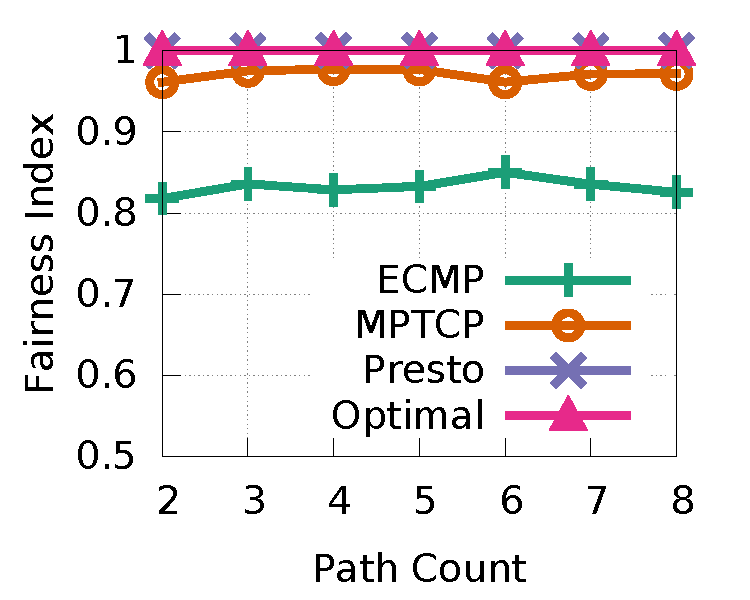
\includegraphics[width=0.45\textwidth]{./figures/scalability_test/scalability_compare_fairness.pdf}
        \caption{Micro benckmark 2 - scalability test. 
		We increase the number of spine switches (i.e., the number of intermediate paths)
                and set the number of flows (host pairs) equal to the number of available paths. 
		Fairness comparison. 20 runs each with each run lasting for 10 seconds.
		Optimal means running TCP on a non-blocking network}
        \label{micro_scalability_test_fairness}
\end{figure}
\fi

\begin{figure}[t]
        \centering
  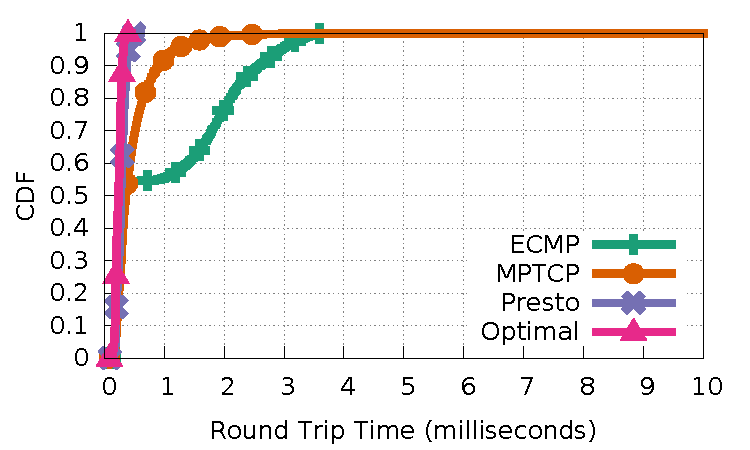
\includegraphics[width=0.45\textwidth]{./figures/scalability_test/scalability_compare_latency.pdf}
        \caption{Round trip time comparison in scalability benchmark. 
		%We increase the number of spine switches (i.e., the number of intermediate paths)
                %and set the number of flows (host pairs) equal to the number of available paths. 
		}
        \label{micro_scalability_test_latency}
\end{figure}


\begin{figure}[t]
        \centering
	\centering
        \begin{subfigure}[b]{0.225\textwidth}
                \centering
		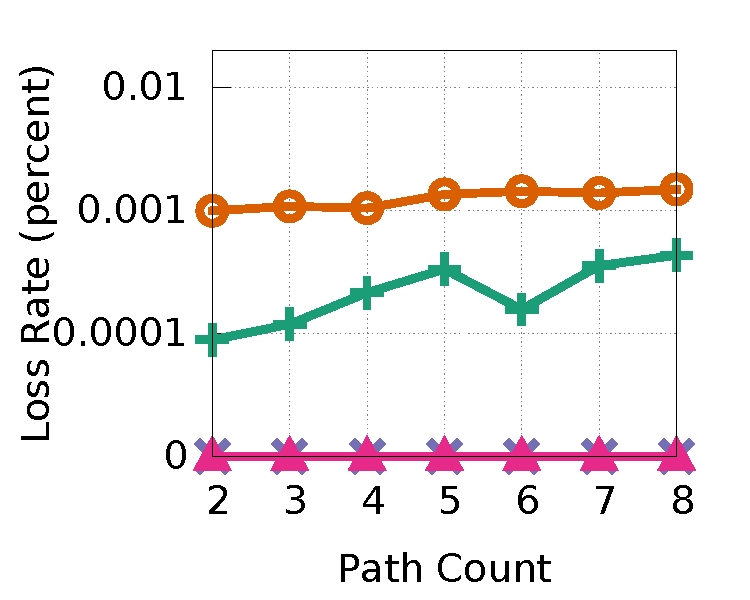
\includegraphics[width=\textwidth]{./figures/scalability_test/scalability_compare_loss.pdf}
		\caption{}
		\label{micro_scalability_test_loss}
        \end{subfigure}
        \begin{subfigure}[b]{0.225\textwidth}
  		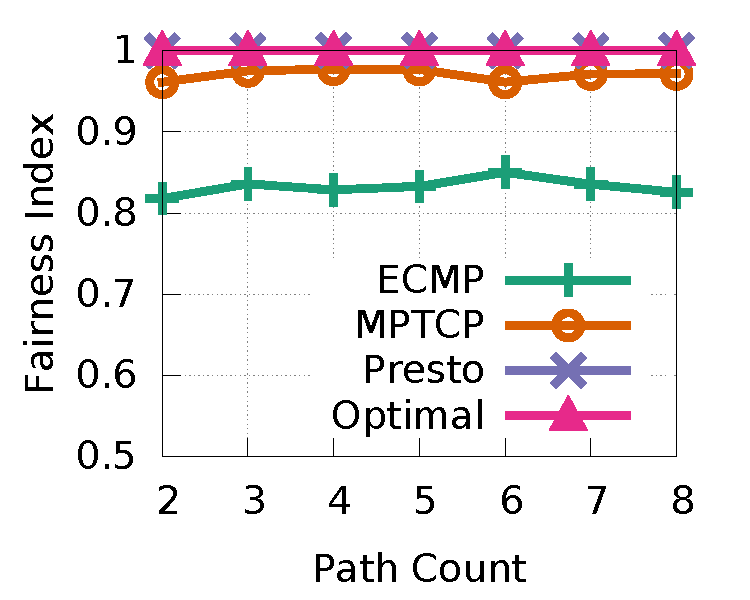
\includegraphics[width=\textwidth]{./figures/scalability_test/scalability_compare_fairness.pdf}
        	\caption{}
        	\label{micro_scalability_test_fairness}
	\end{subfigure}
	\caption{(a) Loss rate and (b) Fairness index comparison in scalability benchmark.}
\end{figure}

\tightparagraph{Presto Scales to Multiple Paths}
We analyze Presto's ability to scale in the number of paths by
setting the number of flows (host pairs) equal to the number of available paths in the topology shown in 
Figure~\ref{micro_scalability_topology}. The number of paths is varied from 2 to 8, and 
Presto always load-balances over all available paths.
Figure~\ref{micro_scalability_test_tput} shows Presto's throughput closely tracks Optimal. 
ECMP (and MPTCP) suffer from lower throughput when flows (or subflows) are
hashed to the same path. Hashing on the same path leads to congestion and thus increased latency, as shown in Figure~\ref{micro_scalability_test_latency}.
Because this topology is non-blocking and Presto load-balances in a near optimal fashion, Presto's latency
is near Optimal. Packet drop rates are presented in Figure~\ref{micro_scalability_test_loss} and show
Presto and Optimal have no loss. MPTCP has higher loss because of its bursty nature~\cite{conga}
and its aggression in the face of loss: when a single loss occurs, only
one subflow reduces its rate. The other schemes are more conservative because a single loss reduces the rate of the whole flow.
Finally, Figure~\ref{micro_scalability_test_fairness} shows Presto, Optimal and MPTCP
achieve almost perfect fairness.
%The underlying reason is that MPTCP makes traffic more bursty~\cite{conga}.


%%%congestion test figures %%%%
\begin{figure}[t]
        \centering
  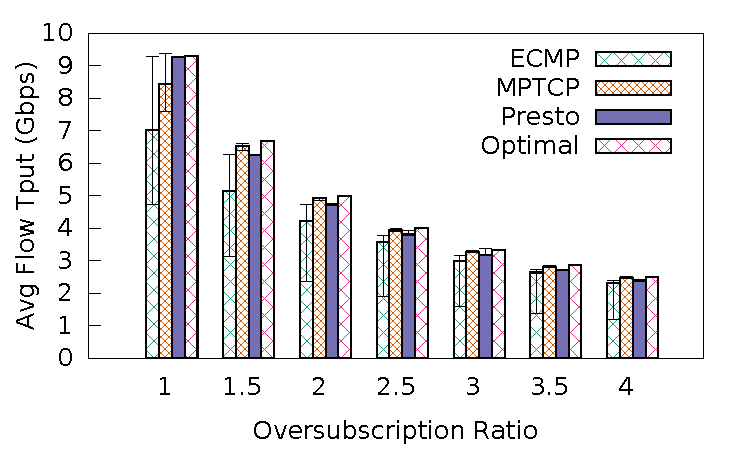
\includegraphics[width=0.45\textwidth]{./figures/congestion_test/congestion_compare_tput_witherrbar.pdf}
        \caption{Throughput comparison in oversubscription benchmark.}
        \label{micro_congestion_test_tput}
\end{figure}


\begin{figure}[t]
        \centering
  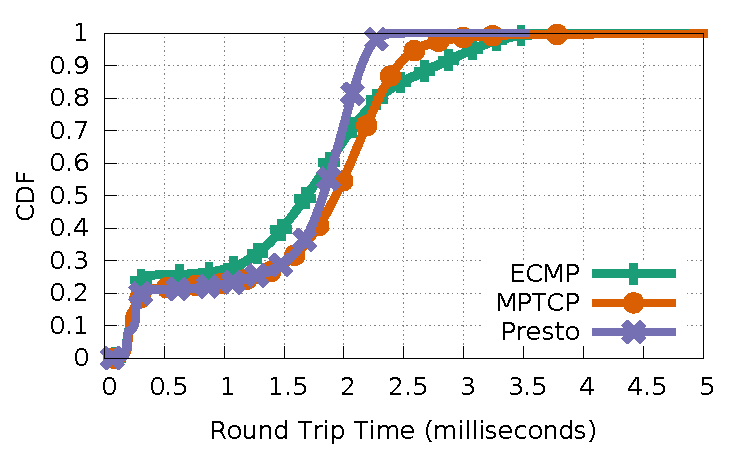
\includegraphics[width=0.45\textwidth]{./figures/congestion_test/congestion_compare_latency.pdf}
        \caption{Round trip time comparison in oversubscription benchmark.
		}
        \label{micro_congestion_test_latency}
\end{figure}



\begin{figure}[t]
        \centering
	\centering
        \begin{subfigure}[b]{0.225\textwidth}
                \centering
		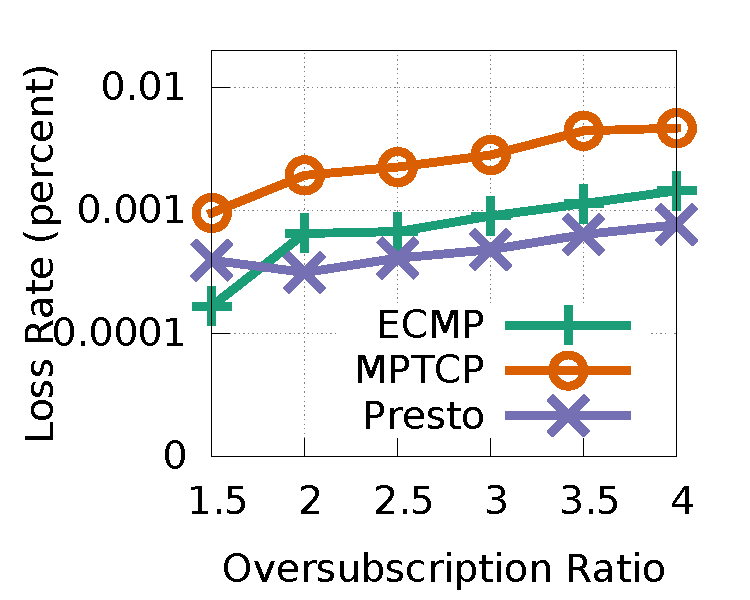
\includegraphics[width=\textwidth]{./figures/congestion_test/congestion_compare_loss.pdf}
		\caption{}
		\label{micro_congestion_test_loss}
	\end{subfigure}
	\begin{subfigure}[b]{0.225\textwidth}
		\centering
  		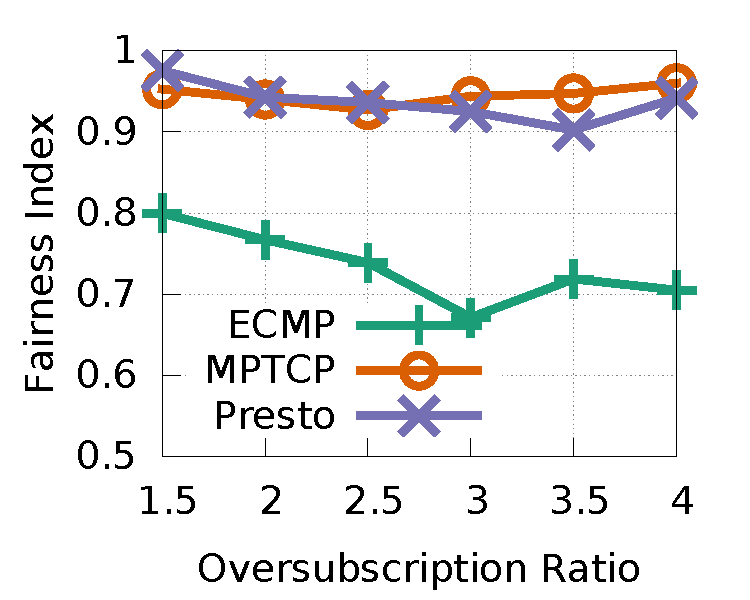
\includegraphics[width=\textwidth]{./figures/congestion_test/congestion_compare_fairness.pdf}
		\caption{}
        \label{micro_congestion_test_fairness}
	\end{subfigure}
	\caption{(a) Loss rate and (b) Fairness index comparison in oversubscription benchmark.}
\end{figure}

\tightparagraph{Presto Handles Congestion Gracefully}
Presto's ability to handle congestion is analyzed by fixing 
the number of spine and leaf switches to 2 and varying
the number of flows (host pairs) from 2 to 8, as shown
in Figure~\ref{micro_congestion_topology}. 
Each flow sends as much as possible, which leads to the network
being oversubscribed by a ratio of 1 (two flows) to 4 (eight flows).
Figure~\ref{micro_congestion_test_tput} shows all schemes track Optimal in highly
oversubscribed environments. ECMP
does poorly under moderate congestion because the limited number of flows can be hashed to the same path.
Presto does no worse in terms of latency (Figure~\ref{micro_congestion_test_latency}) and loss (Figure~\ref{micro_congestion_test_loss}).
The long tail latency for MPTCP is caused by its higher loss rates.
Both Presto and MPTCP have greatly improved fairness compared with ECMP (Figure~\ref{micro_congestion_test_fairness}).

\begin{figure}[!t]
        \centering
  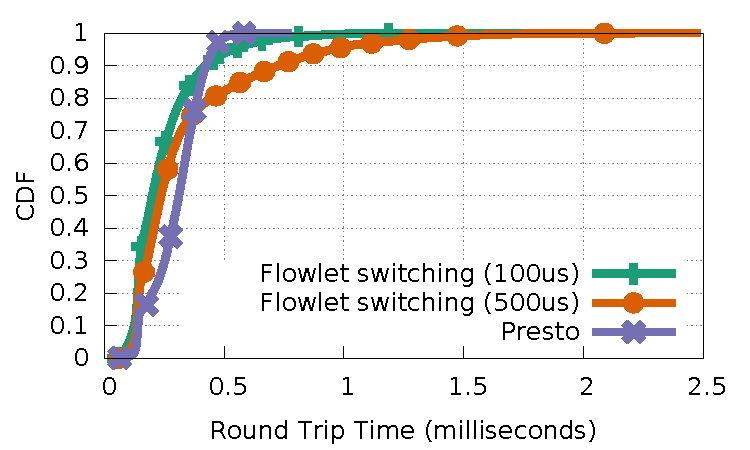
\includegraphics[width=0.45\textwidth]{./figures/flowlets/flowlet_switching/flowlet_presto_compare_sockperf.pdf}
        \caption{Round trip time comparison of flowlet switching and Presto in Stride workload. 
		The throughputs of Flowlet switching with 100 $\mu\text{s}$ gap, 500 $\mu\text{s}$ gap and Presto 
		are 4.3 Gbps, 7.6 Gbps and 9.3 Gbps respectively. }
        \label{micro_flowlet_rtt_compare}
\end{figure}


\tightparagraph{Comparison to Flowlet Switching}
We first implemented a flowlet load-balancing scheme in OVS that detects
inactivity gaps and then schedules flowlets over disjoint paths in a round robin fashion.
%(Presto does this over flowcells instead of flowlets).
The receiver for flowlets uses official GRO.
Our flowlet scheme is not a direct reflection of CONGA because (i) it is not 
congestion-aware and (ii) the flowlets are determined in the software edge
instead of the networking hardware.
Presto is compared to 500 $\mu$s and 100 $\mu$s inactivity timers in
the stride workload on the 2-tier Clos network (Figure~\ref{macro_evaluation_topology}).
The throughput of the schemes are 9.3 Gbps (Presto), 7.6 Gbps (500 $\mu$s), and 4.3 Gbps (100 $\mu$s).
%Switching flowlets on very small timescales, such as 100$\mu$s, provides opportunities to create many flowlets.
%The largest flowlet is only 0.20\% (XX) of the total network traffic, which corresponds to about 5-9 MB in our runs.
%And while small flowlets create an even distribution
%of traffic over the network, significant strain is put on the TCP connection due to packet reordering. 
Analysis of the 100 $\mu$s
network traces show 13\%-29\% packets in the connection are reordered, which means 100 $\mu$s is not enough
time to allow packets to arrive in-order at the destination and thus throughput is severely impacted. Switching flowlets with 500 $\mu$s prevents
most reordering (only 0.03\%-0.5\% packets are reordered), but creates very large flowlets (see Figure~\ref{micro_flowlet_size}). This means
flowlets can still suffer from collisions, which can hurt throughput (note: while not shown here, 500 $\mu$s outperforms ECMP by over 40\%).
Figure~\ref{micro_flowlet_rtt_compare} shows the
latencies. Flowlet 100 $\mu$s has low throughput and hence lower latencies. However, since
its load balancing isn't perfect, it can still cause increased congestion in the tail. Flowlet 500 $\mu$s
also has larger tail latencies because of more pronounced flowlet collisions. As compared to the flowlet
schemes, Presto decreases 99.9$^{th}$ percentile latency by 2x-3.6x.
%Presto, by enforcing small flowlet sizes and explicitly accounting for reordering on the receiver, can obtain near
%line rate throughput with minimal tail latencies. 



%%%%presto 2 mods (ecmp and shaodw MAC) compare
\begin{figure}[!t]
        \centering
  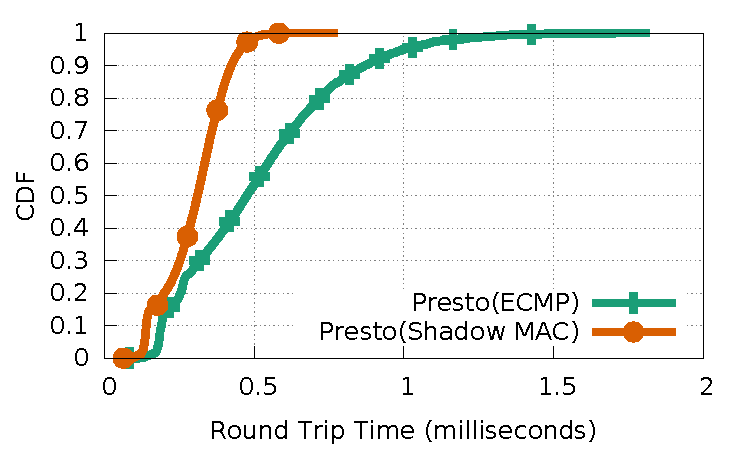
\includegraphics[width=0.45\textwidth]{./figures/presto_compare_2modes/presto_compare_2mods.pdf}
        \caption{Round trip time comparison between Presto + shadow MAC and Presto + ECMP.
		%Compare Presto 2 modes' (Presto over ECMP and Presto over Shadow MAC) performance.
                %Simple 2-tier Clos network with 4 senders and 4 receivers, 4 paths between any host pair.
                %10 seconds per run, 20 runs. Use {\tt nuttcp} to measure throughput. Use {\tt sockperf}
                %to measure latency (RTT).
                %In Presto+ECMP, the average throughput is 7.9 (8.7 if trade latency for tput)
                %Gbps while in Presto+Shadow MAC, the
                %average throughput is 9.3Gbps 
		}
        \label{micro_presto_2mods}
\end{figure}

\tightparagraph{Comparison to Local, Per-Hop Load Balancing}
Presto sends flowcells in a round robin fashion over pre-configured end-to-end paths. An alternative is to
have ECMP hash on flowcell ID and thus provide per-hop load balancing. 
%One way to implement Presto + ECMP is to let vSwitch copy real TCP source port into a pre-allocated TCP option field 
%(\todo{this requires TCP stack allocates the new TCP option before sending to vSwitch}) and 
%encode chunk ID into TCP source port field. Because chunk ID is incremental, ECMP randomly maps chunks into multiple paths. 
We compare Presto + shadow MAC with Presto + ECMP using a stride workload on our testbed. 
Presto + shadow MAC's average throughput is 9.3 Gbps while Presto + ECMP's is 8.9 Gbps.
The round trip time CDF is shown in Figure~\ref{micro_presto_2mods}. 
Presto + shadow MAC gives better latency performance compared with Presto + ECMP. 
The performance difference comes from the fact that Presto + shadow MAC provides 
better fine-grained flowcell load balancing because 
randomization in per-hop multipathing can lead to corner cases where
a large fraction of flowcells get sent to the same link over a small timescale by multiple flows. This transient congestion
can lead to increased buffer occupancy and higher delays.

\subsection{Macrobenchmarks}
\label{macro}

%%%%%%%%%%using figures to present incast: tput, fariness, droprate, TCP RTT
\begin{figure}[t]
        \centering
        \begin{subfigure}[b]{0.225\textwidth}
                \centering
                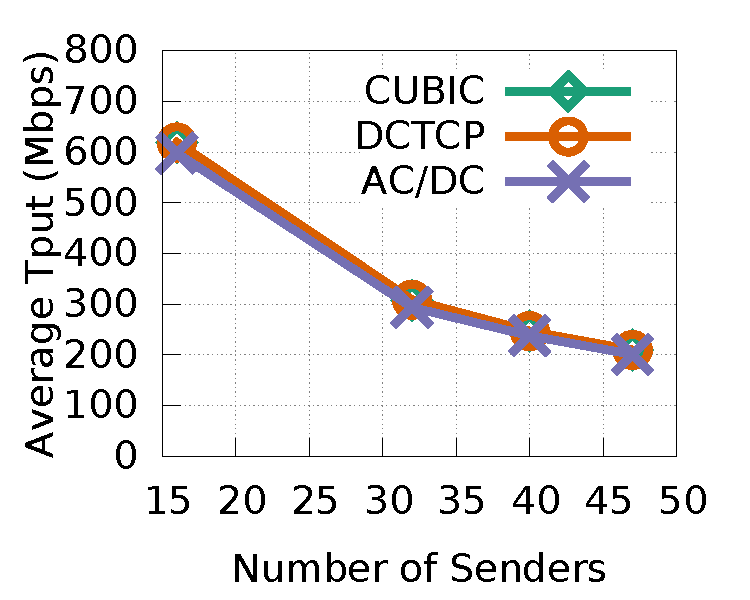
\includegraphics[width=\textwidth]{figures/incast/plots9k/incast_tput_vary_sender.pdf}
                \caption{average throughput.}
                \label{incast_9k_tput}
        \end{subfigure}
        \begin{subfigure}[b]{0.225\textwidth}
                \centering
                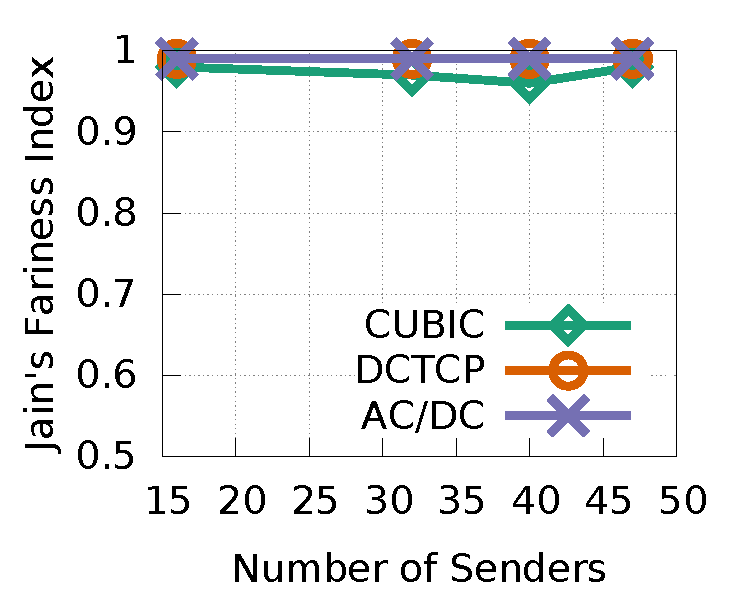
\includegraphics[width=\textwidth]{figures/incast/plots9k/incast_fairness_vary_sender.pdf}
                \caption{fairness.}
                \label{incast_9k_fariness}
        \end{subfigure}
        \caption{Many to one incast: throughput and fairness.}
        \label{incast_9k_tput_fairness}
\end{figure}

\begin{figure*}[!t]
        \centering
        \begin{subfigure}[b]{0.33\textwidth}
                \centering
                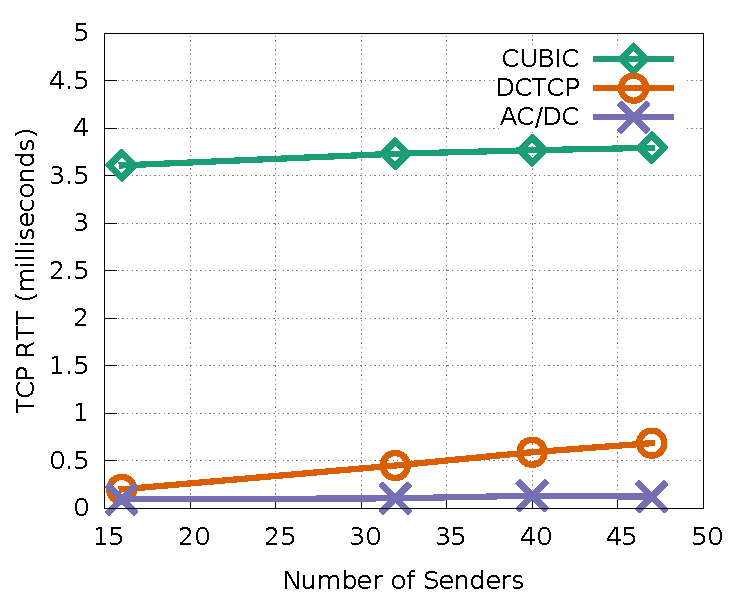
\includegraphics[width=\textwidth]{figures/incast/plots9k/incast_sockperf50th_vary_sender.pdf}
                \caption{50$^{th}$ percentile RTT ($\mu$s).}
                \label{incast_9k_50th_sockperf}
        \end{subfigure}
        \begin{subfigure}[b]{0.33\textwidth}
                \centering
                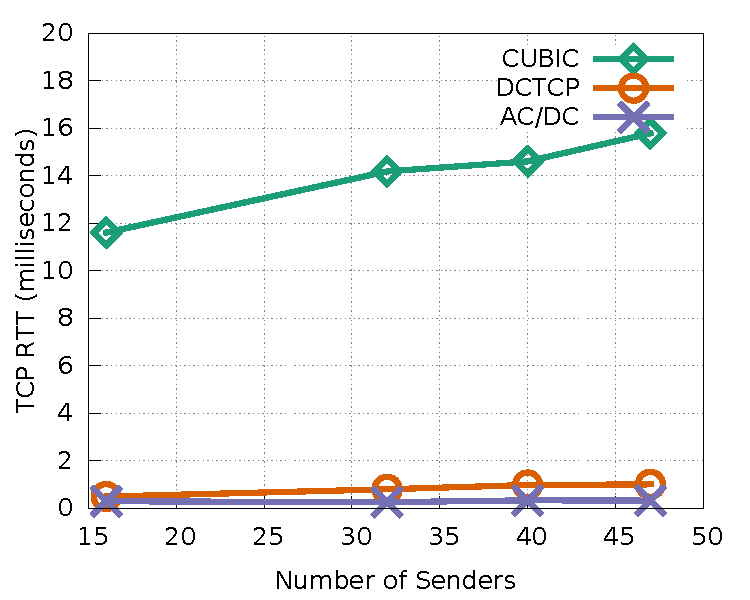
\includegraphics[width=\textwidth]{figures/incast/plots9k/incast_sockperf999th_vary_sender.pdf}
                \caption{99.9$^{th}$ percentile RTT ($\mu$s).}
                \label{incast_9k_999th_sockperf}
        \end{subfigure}
        \begin{subfigure}[b]{0.33\textwidth}
                \centering
                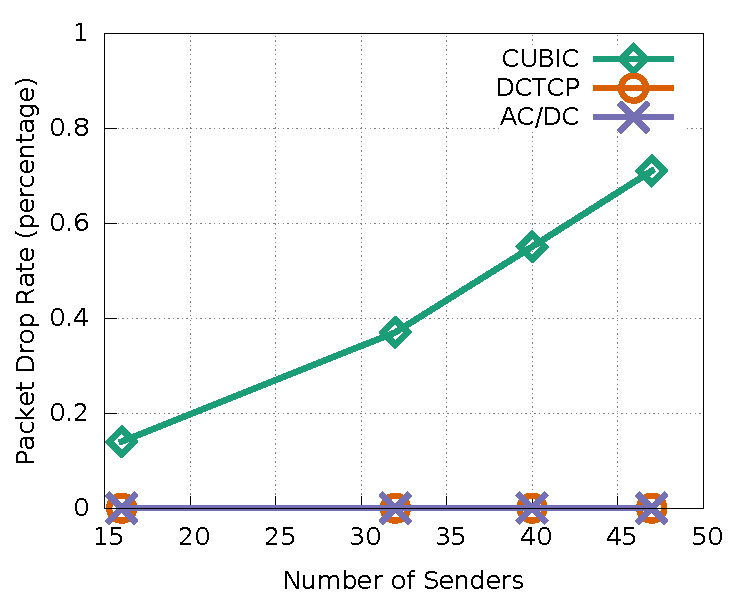
\includegraphics[width=\textwidth]{figures/incast/plots9k/incast_droprate_vary_sender.pdf}
                \caption{packet drop rate.}
                \label{incast_9k_droprate}
        \end{subfigure}
        \caption{Many to one incast: RTT and packet drop rate.}
        \label{incast_9k_sockperf_droprate}
\end{figure*}


\begin{figure}[t]
        \centering
  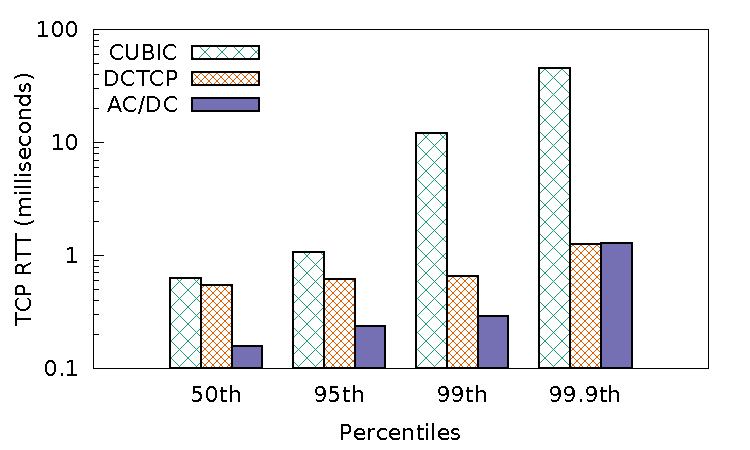
\includegraphics[width=0.45\textwidth]{figures/incast/pressure/incast_pressure_compare_sockperf.pdf}
        \caption{TCP RTT measurement results when almost all ports are congested.}
        \label{sockperf_pressure_incast}
\end{figure}

%
%

\iffalse
\begin{figure*}[!t]
        \centering
        \begin{subfigure}[b]{0.45\textwidth}
                \centering
                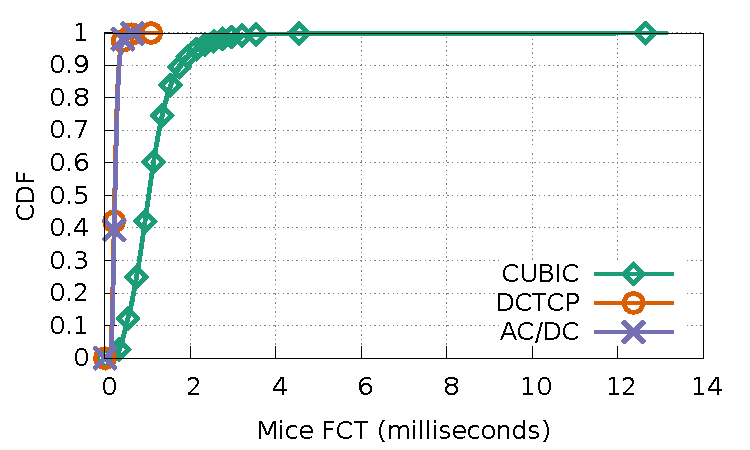
\includegraphics[width=\textwidth]{figures/macro_benchmarks/macro_4stride/stride4_mice16KB_fct.pdf}
                \caption{Mice flow completion times.}
                \label{macro_4stride_mice_fct}
        \end{subfigure}
        \begin{subfigure}[b]{0.45\textwidth}
                \centering
                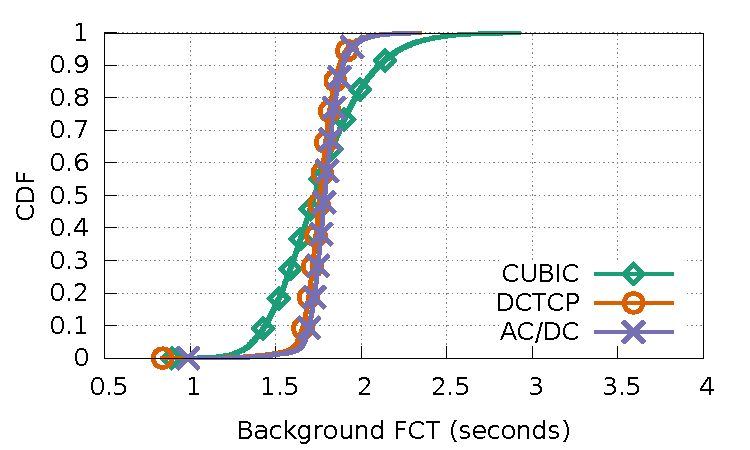
\includegraphics[width=\textwidth]{figures/macro_benchmarks/macro_4stride/stride4_big512MB_fct.pdf}
                \caption{Background flow completion times.}
                \label{macro_4stride_background_fct}
        \end{subfigure}
        \caption{CDF of mice and background FCTs in concurrent stride workload.}
        \label{macro_4stride_fct}
\end{figure*}

\begin{figure*}[!t]
        \centering
        \begin{subfigure}[b]{0.45\textwidth}
                \centering
                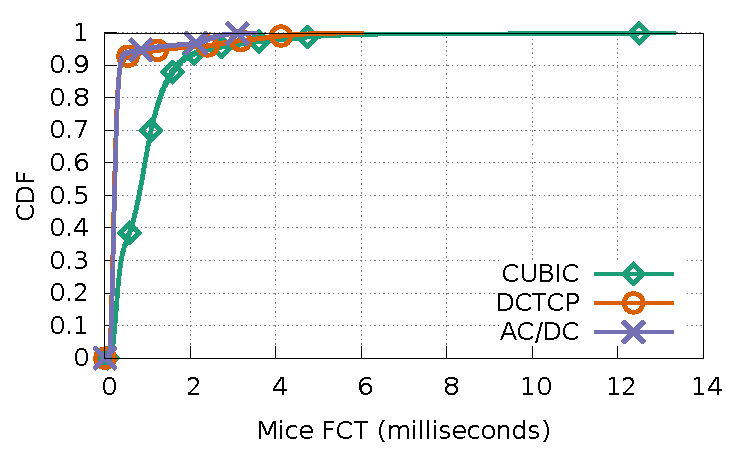
\includegraphics[width=\textwidth]{figures/macro_benchmarks/shuffle_17hosts/shuffle_mice16KB_fct.pdf}
                \caption{Mice flow completion times.}
                \label{macro_shuffle_mice_fct}
        \end{subfigure}
        \begin{subfigure}[b]{0.45\textwidth}
                \centering
                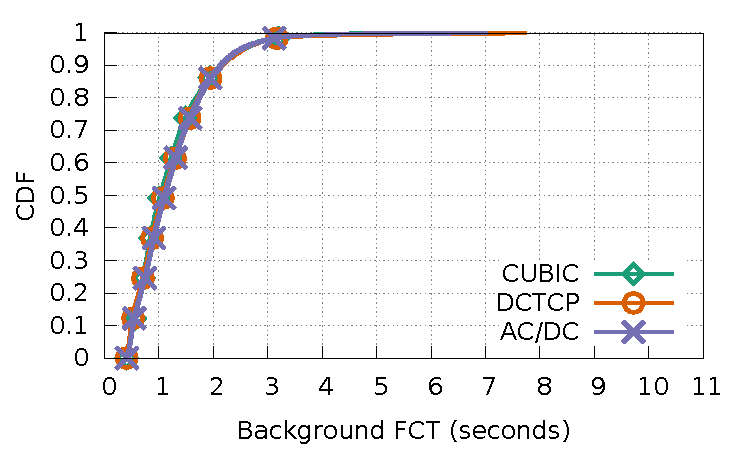
\includegraphics[width=\textwidth]{figures/macro_benchmarks/shuffle_17hosts/shuffle_big512MB_fct.pdf}
                \caption{Background flow completion times.}
                \label{macro_shuffle_background_fct}
        \end{subfigure}
        \caption{CDF of mice and background FCTs in shuffle workload.}
        \label{macro_shuffle_fct}
\end{figure*}

\begin{figure*}[!t]
        \centering
        \begin{subfigure}[b]{0.45\textwidth}
                \centering
                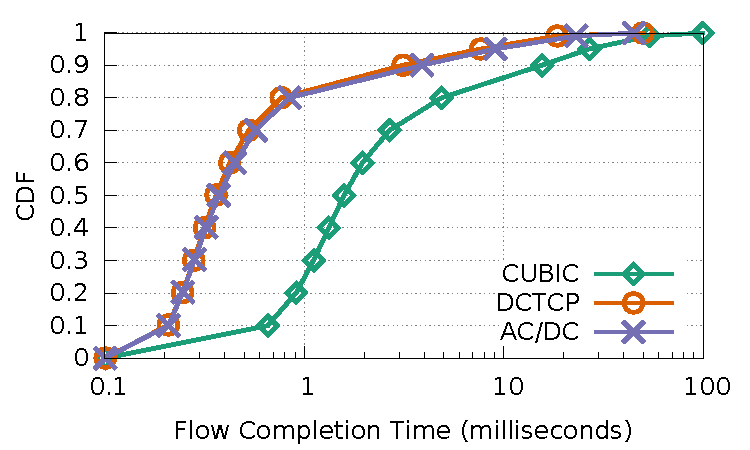
\includegraphics[width=\textwidth]{figures/macro_benchmarks/trace-driven/trace_driven_workload_dctcp_senders5_10points.pdf}
                \caption{Web-search workload.}
                \label{trace-driven-searching-fct}
        \end{subfigure}
        \begin{subfigure}[b]{0.45\textwidth}
                \centering
                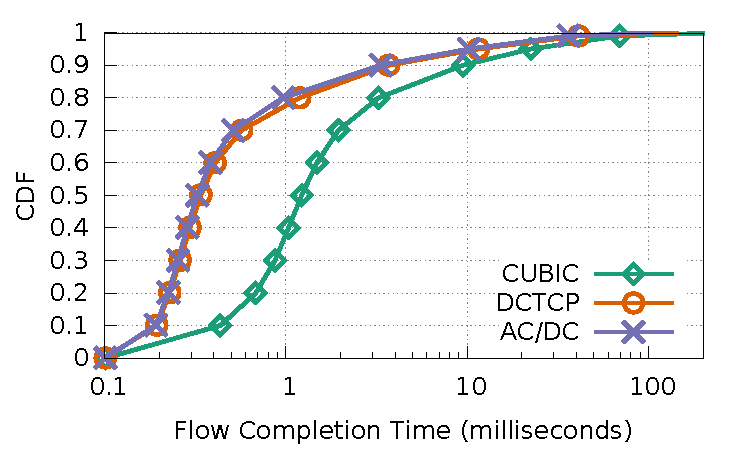
\includegraphics[width=\textwidth]{figures/macro_benchmarks/trace-driven/trace_driven_workload_conga_senders5_10points.pdf}
                \caption{Data-mining workload.}
                \label{trace-driven-data-mining-fct}
        \end{subfigure}
        \caption{CDF of mice flow's (<10KB) FCT in web-search and data-mining workloads.}
        \label{macro-trace-driven-fct}
\end{figure*}
\fi


In this section we attach all servers to a single switch and
run a variety of well-known workloads to better understand
how well~\acdc{} can track DCTCP's performance. Experiments are run for 10 minutes. A simple TCP application
sends messages of specified sizes to measure flow completion times.

\tightparagraph{Incast}
In this section, we evaluate incast scenarios.
To scale the experiment, 17 physical servers are equipped with four NICs each
and one flow is allocated per NIC.
In this way, incast can support up to 47-to-1 fan-in (our switch only has 48 ports).
We measure the extent of incast by increasing the number of concurrent senders to 16, 32, 40 and 47.
Figure~\ref{incast_9k_tput_fairness} shows throughput and fairness results.
Both DCTCP and \acdc{} get comparable throughput as CUBIC and both offer a fairness index greater than 0.99.
Figure~\ref{incast_9k_sockperf_droprate} shows the RTT and packet drop rate results.
When there are 47 concurrent senders, DCTCP can reduce median RTT by 82\% and \acdc{} can reduce by 97\%;
DCTCP can reduce 99.9$^{th}$ percentile RTT by 94\% and \acdc{} can reduce by 98\%.
Both DCTCP and \acdc{} have 0\% packet drop rate. It is curious that~\acdc{}’s
performance is better than DCTCP when the number of senders increases (Figure~\ref{incast_9k_50th_sockperf}).
The Linux DCTCP code puts a lower bound of 2 packets on \cwnd{}.
In incast, we have up to 47 concurrent competing flows and
the network's MTU size is 9kB. In this case, the lower bound is too high,
so DCTCP's RTT increases gradually with the number of senders.
This issue was also found in~\cite{judd2015nsdi}.~\acdc{} controls \rwnd{} (which is in bytes)
instead of \cwnd{} (which is in packets) and \rwnd{}'s lowest value can be much smaller than 2*MSS.
We verified modifying~\acdc{}'s lower bound caused identical behavior.

The second test checks whether \acdc{} can interact well with the switch's dynamic
buffer allocation scheme. To this end, we aim to congest every switch port.
The 48 NICs are split into 2 groups: group $A$ and $B$.
Group $A$ has 46 NICs and $B$ has 2 (denoted $B_1$ and $B_2$).
Each of the 46 NICs in $A$ sends and receives 4 concurrent flows within $A$
(\ie{}, NIC $i$ sends to [$i+1$, $i+4$] mod 46).
Meanwhile, all of the NICs in $A$ send to $B_1$, creating a 46-to-1 incast.
This workload congests 47 out of 48 switch ports.
We measure the RTT between $B_2$ and $B_1$ (i.e., RTT of the traffic traversing the most congested port) and
the results are shown in Figure~\ref{sockperf_pressure_incast}.
The average throughputs for CUBIC, DCTCP, and~\acdc{} are 214, 214 and 201 Mbps respectively,
all with a fairness index greater than 0.98.
CUBIC has an average drop rate of 0.34\% but the most congested port has a drop rate as high as 4\%.
This is why the 99.9$^{th}$ percentile RTT for CUBIC is very high.
The packet drop rate for both DCTCP and~\acdc{} is 0\%.

\begin{figure*}[!t]
        \centering
        \begin{subfigure}[b]{0.45\textwidth}
                \centering
                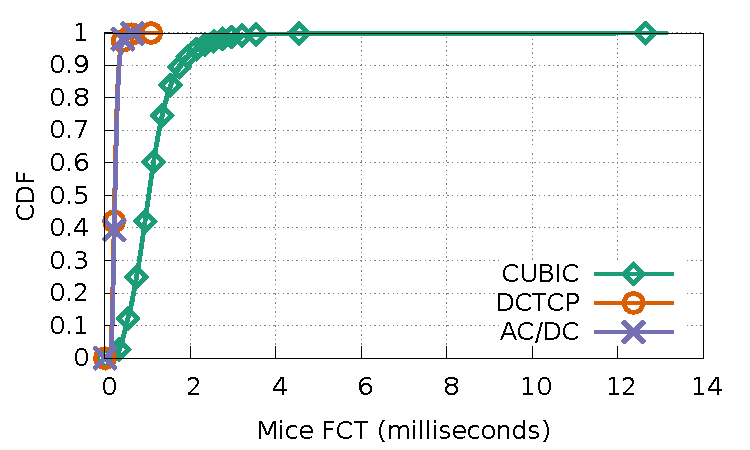
\includegraphics[width=\textwidth]{figures/macro_benchmarks/macro_4stride/stride4_mice16KB_fct.pdf}
                \caption{Mice flow completion times.}
                \label{macro_4stride_mice_fct}
        \end{subfigure}
        \begin{subfigure}[b]{0.45\textwidth}
                \centering
                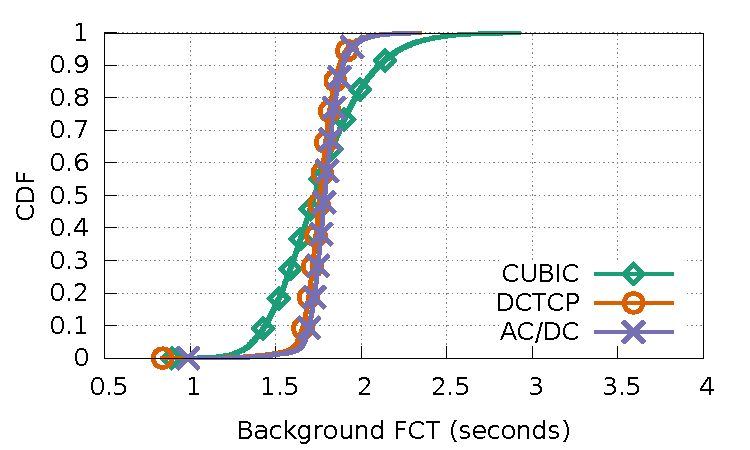
\includegraphics[width=\textwidth]{figures/macro_benchmarks/macro_4stride/stride4_big512MB_fct.pdf}
                \caption{Background flow completion times.}
                \label{macro_4stride_background_fct}
        \end{subfigure}
        \caption{CDF of mice and background FCTs in concurrent stride workload.}
        \label{macro_4stride_fct}
\end{figure*}

\begin{figure*}[!t]
        \centering
        \begin{subfigure}[b]{0.45\textwidth}
                \centering
                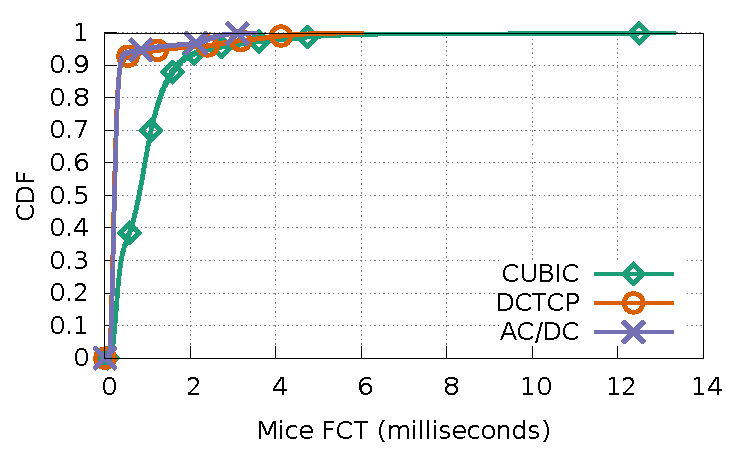
\includegraphics[width=\textwidth]{figures/macro_benchmarks/shuffle_17hosts/shuffle_mice16KB_fct.pdf}
                \caption{Mice flow completion times.}
                \label{macro_shuffle_mice_fct}
        \end{subfigure}
        \begin{subfigure}[b]{0.45\textwidth}
                \centering
                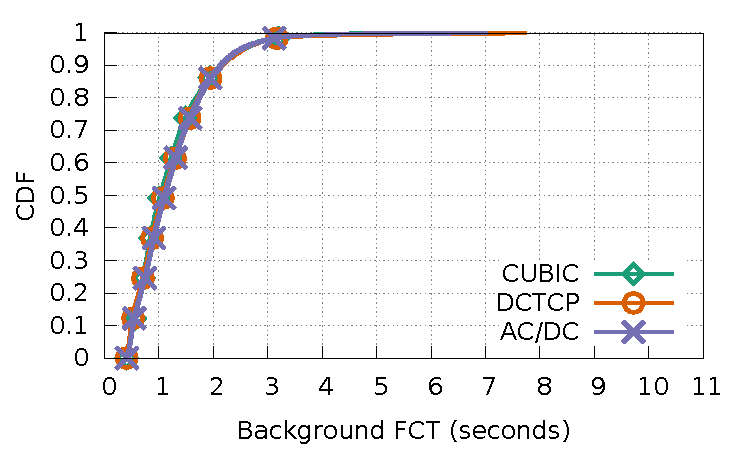
\includegraphics[width=\textwidth]{figures/macro_benchmarks/shuffle_17hosts/shuffle_big512MB_fct.pdf}
                \caption{Background flow completion times.}
                \label{macro_shuffle_background_fct}
        \end{subfigure}
        \caption{CDF of mice and background FCTs in shuffle workload.}
        \label{macro_shuffle_fct}
\end{figure*}

\begin{figure*}[!t]
        \centering
        \begin{subfigure}[b]{0.45\textwidth}
                \centering
                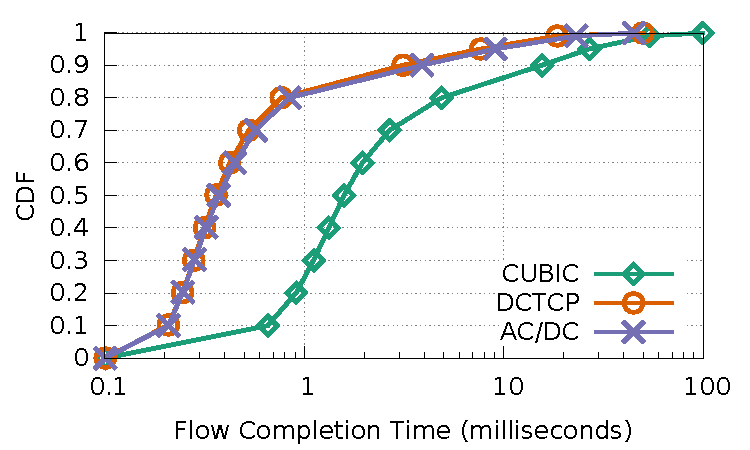
\includegraphics[width=\textwidth]{figures/macro_benchmarks/trace-driven/trace_driven_workload_dctcp_senders5_10points.pdf}
                \caption{Web-search workload.}
                \label{trace-driven-searching-fct}
        \end{subfigure}
        \begin{subfigure}[b]{0.45\textwidth}
                \centering
                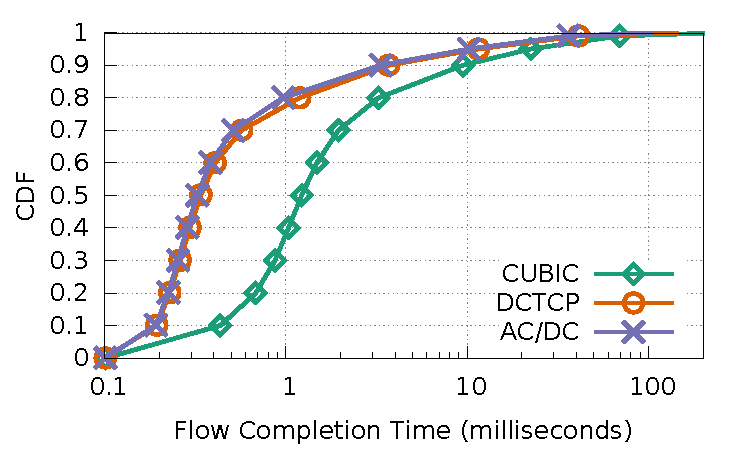
\includegraphics[width=\textwidth]{figures/macro_benchmarks/trace-driven/trace_driven_workload_conga_senders5_10points.pdf}
                \caption{Data-mining workload.}
                \label{trace-driven-data-mining-fct}
        \end{subfigure}
        \caption{CDF of mice flow's (<10KB) FCT in web-search and data-mining workloads.}
        \label{macro-trace-driven-fct}
\end{figure*}

\tightparagraph{Concurrent stride workload}
In concurrent stride, 17 servers are attached to a single switch.
Each server $i$ sends a 512MB flow to servers [$i+1$, $i+4$] mod 17 in sequential fashion
to emulate background traffic.
Simultaneously, each server $i$ sends 16KB messages every 100 ms to 
server $(i+8)$ mod 17.
The FCT for small flows (16KB) and background flows (512MB) are shown 
in Figure~\ref{macro_4stride_fct}. For small flows, DCTCP and \acdc{} 
reduce the median FCT by 77\% and 76\% respectively. 
At the 99.9$^{th}$ percentile, DCTCP and \acdc{} reduce FCT by 91\% and 93\%, respectively.
For background flows, DCTCP and \acdc{} offer similar completion times.
CUBIC has longer background FCT because its fairness is not as 
good as DCTCP and \acdc{}.


\tightparagraph{Shuffle workload}
In shuffle, each server sends 512MB to every other server in random order. 
A sender sends at most 2 flows simultaneously and when
a transfer is finished, the next one is started until 
all transfers complete.
Every server $i$ also sends a 16 KB message to server $(i+8)$ mod 17 
every 100 ms. This workload is repeated for 30 runs.
The FCT for each type of flow is shown in Figure~\ref{macro_shuffle_fct}.
For small flows, DCTCP and \acdc{} reduce median FCT by
72\% and 71\% when compared to CUBIC. 
At the 99.9$^{th}$ percentile, DCTCP and \acdc{} 
reduce FCTs by 55\% and 73\% respectively.
For large flows, CUBIC, DCTCP and \acdc{} have almost identical performance.


\tightparagraph{Trace-driven workloads}
Finally, we run trace-driven workloads. 
An application on each server builds a long-lived TCP connection with every other server.
Message sizes are sampled from a trace and sent to a random destination in sequential fashion. Five
concurrent applications on each server are run to increase network load. Message
sizes are sampled from a web-search~\cite{alizadeh2011data}
and a data-mining workload~\cite{greenberg2009vl2,alizadeh2014conga}, whose flow size distribution has a heavier tail.
Figure~\ref{macro-trace-driven-fct} shows a CDF of FCTs for mice flows (smaller than 10KB) 
in the web-search and data-mining workloads.
In the web-search workload,
DCTCP and \acdc{} reduce median FCTs by 77\% and 76\%, respectively. 
At the 99.9$^{th}$ percentile, DCTCP and \acdc{} reduce FCTs by 50\% and 55\%, respectively.
In the data-mining workload, DCTCP and \acdc{} reduce median FCTs by 72\% and 73\%, respectively. 
At the 99.9$^{th}$ percentile, DCTCP and \acdc{} reduce FCTs by 36\% and 53\% respectively.  
%In both workloads, DCTCP and \acdc{} improve the fraction of mice flows that finish 
%in 1 millisecond significantly (from 20\%/30\% to 80\%).

\tightparagraph{Evaluation summary}
The results validate that congestion control can be accurately implemented in the vSwitch.
~\acdc{} tracks the performance of an unmodified host DCTCP stack
over a variety of workloads with little computational overhead.
Furthermore,~\acdc{} provides this functionality over 
various host TCP congestion control configurations. 


%\section{Discussion}
\label{discuss}

\tightparagraph{UDP traffic} How to handle. 
Mention VxLAN traffic too.
\keqiang{and IPsec}

\tightparagraph{No vSwitch} 
\keqiang{title should be hypervisor-bypass?}
Use middleboxes (for DB server).
Use NIC (for SR-IOV).
Hypervisor bypass (e.g., SR-IOV), where TCP traffic is sent to the NIC directly without 
going through hypervisor. First, as noted by~\cite{shieh2011sharing}, ``loss of the security and 
manageability features provided by the software virtual switch has limited 
the deployment of direct I/O NICs in public clouds''. Second, based on techniques like Intel 
DPDK~\cite{intel-dpdk} and ``smart NICs''~\cite{cavium-nic,netronome-nic}, we believe that low latency 
congestion control enforcement schemes like \acdc{} can also be 
employed for hypervisor bypass use cases.
We need to worry about legacy systems and non-VM systems. For instance, a database or storage device that may not have OVS installed on it.
We need to talk about either a middlebox or that this percentage of traffic is low? Or implement in NIC (especially one with OVS offload?).

\tightparagraph{North-South traffic.}
Transport enforcement should be only be done for east west traffic, so if the tenant tuned their stack's
congestion control algorithm for wide-area networks, their north sourth traffic is not affected and their 
congestion control scheme can still achieve good performance.

\keqiang{todos: some figures do not read well on printed paper}
\keqiang{todos: sometimes, when we refer a section, we say ``Section X'', sometimes, we use the 
dollar sign, we should unify them}

%
%Byzantine VM.
%
%Other names: ACDCTCP, LiquidSwitch, LiquidEdge
%
%In CPU overhead measurement, we need to 
%mention ovs add 1 widecard rule. That means we isolated the overhead of 
%OVS itself when it has many flows in its flow table (probably it does not matter
%at the end of the day, because we measured the CPU usage of the whole system).
%
%People may say window-based congestion control is burty. TIMELY operates 
%on TCP segments in order to reduce CPU overhead. Therefore, TIMELY is also
%busty. In TIMELY, they mentioned they can leverage a hybrid scheme, that is
%using software to control large segments and use hardware rate limiter to
%reduce burstyness.
%
%Create loss and check how DCTCP and our scheme treates packet losses (revisit it after we finish incast 
%and macrobenchmarks).
%
%One more microbenchmark on the Dumbbell topology: different servers have different transport, so the
%throughput fairness among different transports (e.g., start cubic, start New Reno, start dctcp).
%
%A point that is missing in DCTCP and NSDI paper is that they did not mention how the switch should be
%configured to handle non-TCP traffic. Note non-TCP traffic such as DNS (UDP 53) and ARP, ICMP etc
%are also important. We found that if we did not specify how the switch handle the non-TCP traffic,
%then this kind of non-TCP traffic can be easily dropped by the switch. We found ARP traffic is dropped
%by the switch such that DCTCP flows stall. Hence, we think it is better to put non-TCP traffic
%into a different queue when we apply WRED/ECN on the switches.
%
%This work offers low latency for ``hetergeneous networks" where different entities can 
%run different kinds of
%transport congestion control schemes. A few examples of such hetergeneous networks: public 
%datacenters where tenants can set up their own VMs (e.g., AWS), or tenants can rent their bare metal
%machines (e.g., SoftLayer), or certain groups (even within a single organization) 
%have to use traditional transports due to compatibility of legacy applications (NSDI's Judd said this), or
%incremental deployment is undergoing. 
%To ensure a pure low latency datacenter network, a universal transport enforcement scheme is required. 
%Two challenges to implement such a transport enforcement scheme are scalability and low overhead. 
%The transport enformancement scheme proposed here meet the two metrics (as shown in our experiments) while
%providing nice network performance (throughput, latency and packet drop rate). This scheme is 
%compatible with any kind of TCP stack. Finally, the scheme we propose solves the co-existence issue of 
%ECT (ECN Capable Transport) and non-ECT, which is a critical deployment hurdle for DCTCP-like transports.
%
%Macrobenchmark plan: 18 hosts, 6 switches, ECMP configured. The network oversubscription ratio is 2:1.
%Run all-to-all traffic for a long time (e.g., 1 hours). Show total throughput and TCP RTT and packet drop 
%rate.
%
%QoS can be implemented too?
%
%
%
%When we try to launch an instance in EC2: ``An AMI is a template that contains the software 
%configuration (operating system, application server, and applications) required to launch your instance. 
%You can select an AMI provided by AWS, our user community, or the AWS Marketplace; 
%or you can select one of your own AMIs''. Default is CUBIC for most Linux images, Window Servers can
%have NewReno, Compound TCP (CTCP)~\cite{tan2006compound} and DCTCP. 
%Users can tweak congestion control algorithms to optimize network performance for their target scenarios. 
%
%Section talking about how to implement other CC schemes: TIMELY, PERC, Vegas, etc.
%
%EJR: VXLAN, UDP, TCP stack statistics for Cloud?
%
%ECT and non-ECT: througput unfairness, long RTT, connection establishment..
%
%
%EyeQ, Seawall, NetShare, Silo, SecondNet, Oktopus etc. Our work did not provide bandwidth allocation property. 
%This work focused on reducing in-network queuing latency caused by VM TCP stacks. 
%We show how this goal can be done using a simple and elegant solution.
%Yes, if an VM opens more connections than another, that VM gains more bandwidth. 
%But, there are proposals which try to provide proper bandwidth allocation when multiple end-points compete 
%at the sender side or receiver side. Those works and this work are complementary. 
%To the best of our knowledge, today's cloud providers have not provide strong bandwidth guarantees 
%(for example, AWS only roughly classify VMs instances' network performance into 
%``low to moderate", ``moderate", ``high" and ``10 Gigabit"categories).
%
%talk about containers?

\section{Related Work}
\label{related}
This section discusses different classes of related work.

\tightparagraph{Congestion control for DCNs}
\crs{Rather than proposing a new congestion control algorithm, our work investigates if congestion control can be moved to the vSwitch.
Thus, many of the following schemes are complimentary.}
DCTCP~\cite{alizadeh2011data} is a seminal TCP variant for datacenter networks.
Judd~\cite{judd2015nsdi} proposed simple yet practical fixes to enable DCTCP in production networks.
TCP-Bolt~\cite{stephens2014practical} is a variant of DCTCP for PFC-enabled lossless Ethernet.
%DCQCN~\cite{zhu2015congestion} is a rate-based congestion control scheme implemented in NICs
%for QCN-based~\cite{qcn} RDMA deployments.
DCQCN~\cite{zhu2015congestion} is a rate-based congestion control scheme (built on DCTCP and QCN) to
support RDMA deployments in PFC-enabled lossless networks.
TIMELY~\cite{mittal2015timely} and DX~\cite{lee2015accurate} 
use accurate network latency as the signal to perform congestion control.
TCP ex Machina~\cite{winstein2013tcp} uses computer-generated congestion control rules.
PERC~\cite{jose2015high} proposes proactive congestion control to improve convergence.
ICTCP's~\cite{wu2010ictcp} receiver monitors incoming TCP flows and 
modifies~\rwnd{} to mitigate the impact of incast, but this cannot
provide generalized congestion control like~\acdc{}.
Finally, efforts~\cite{dell-toe,chelsio-toe} to 
implement TCP Offload Engine (TOE) in specialized NICs are not widely deployed for reasons noted in~\cite{mogul2003tcp,linux-toe}.
%~\acdc{} is designed to work with commodity NICs. 

\tightparagraph{Bandwidth allocation} Many bandwidth allocation schemes have been proposed.
Gatekeeper~\cite{rodrigues2011gatekeeper} and EyeQ~\cite{jeyakumar2013eyeq} abstract the network as a single
switch and provide bandwidth guarantees by managing each server's access link.
Oktopus~\cite{Ballani2011oktopus} provides fixed performance guarantees within virtual clusters.
SecondNet~\cite{Guo2010Secondnet} enables virtual datacenters with static bandwidth guarantees.
Proteus~\cite{Xie2012Proteus} allocates bandwidth for applications with dynamic demands.
Seawall~\cite{shieh2011sharing} provides bandwidth proportional to a defined weight by
forcing traffic through congestion-based edge-to-edge tunnels. 
NetShare~\cite{Lam2012NetShare} utilizes hierarchical weighted max-min fair sharing to tune relative bandwidth allocation for services.
FairCloud~\cite{Popa2012Faircloud} identifies trade-offs in minimum
guarantees, proportionality and high utilization, and designs schemes over this space.
Silo~\cite{jang2015silo} provides guaranteed bandwidth, delay and burst allowances through a novel VM placement and admission 
algorithm, coupled with a fine-grained packet pacer. As discussed in~\cref{background}, 
~\acdc{} is largely complimentary to these schemes because it is a transport-level solution.

\tightparagraph{Rate limiters} 
SENIC~\cite{niranjan2013fastrak} 
identifies the limitations of NIC hardware rate limiters (\ie{}, not scalable) and 
software rate limiters (\ie{}, high CPU overhead) and uses the CPU to enqueue packets 
in host memory and the NIC. Silo's pacer injects void packets into 
an original packet sequence to achieve pacing. FasTrack~\cite{niranjan2013fastrak} offloads
functionality from the server into the switch for certain flows.~\acdc{} prevents
TCP flows from sending in the first place and can be used in conjunction with these
schemes.


\tightparagraph{Low latency DCNs}
Many schemes have been proposed to reduce latency in datacenter networks.
HULL~\cite{alizadeh2012less} uses phantom queues to leave bandwidth headroom to support low latency.
pFabric~\cite{alizadeh2013pfabric} is a clean-slate
design which utilizes priority and minimal switch buffering to achieve low latency.
Fastpass~\cite{perry2014fastpass} uses a centralized arbiter to
perform per-packet level scheduling.
QJUMP~\cite{qjump} uses priority queueing and rate limiting to
bound latency. Traffic engineering~\cite{al2010hedera,rasley2014planck} and 
load balancing~\cite{alizadeh2014conga,he2015presto,ghorbani2015micro} can also
reduce latency. Because~\acdc{} works on the transport level, it is
largely complimentary to these works.

\tightparagraph{Performance-enhancing proxies}
Several schemes improve end-to-end protocol performance via a middlebox
or proxy~\cite{RFC3449,RFC3115,balakrishnan2008maelstrom,davern2011httpep,balakrishnan1995improving}.
\acdc{} fits into this class of works, but is unique in providing a mechanism
to alter a VM's TCP congestion control algorithm by modifying the vSwitch.

\tightparagraph{Virtualized congestion control}
\crs{vCC~\cite{vcc} is a concurrently designed system that shares~\acdc{}'s goals and some of its design details.
The paper is complementary in that some items not addressed in this work are presented, such as a more detailed
analysis of the ECN-coexistence problem, an exploration of the design space, and a theoretical proof of
virtualized congestion control's correctness. Our paper provides an in-depth design and thorough evaluation of
a DCTCP-based virtualized congestion control algorithm on a 10 Gbps testbed.
}

\section{Conclusion}
\label{sec:conclusion}

Our measurements across four OpenFlow-based switches show
that the latencies underlying the generation of control messages
(pkt\_in’s) and execution of control operations (flow\_mod’s) can
be quite high, and variable. We find that the underlying causes
are linked both to software inefficiencies, as well as pathological
interactions between switch hardware properties (shared resources
and how forwarding rules are organized) and the control operation
workload (the order of operations issues, and concurrent switch
activities). Finally, to mitigate the challenges these latencies create
for SDN in supporting critical management applications, we
present three measurement-driven techniques. Our evaluation shows
that these mechanisms can tame flow setup latencies effectively.


\balance
{%\scriptsize
\setlength{\bibsep}{0.5pt}
\raggedright
\bibliographystyle{abbrv}
\bibliography{refer}
}

\end{document}
